% ****************************************************************************************************
% Master Thesis Template
% Faculty of Electrical Engineering and Information Technology
% Darmstadt University of Applied Sciences
% KU, 15.9.2020


% ****************************************************************************************************
% Set your personel data here
% ****************************************************************************************************

\newcommand{\myTitle}{Camera pose and Keyframe trajectory estimation on Unmanned Aerial Vehicles\xspace}
\newcommand{\myDegree}{Master of Science (M.Sc.)\xspace}
\newcommand{\myName}{Shreyas Manjunath\xspace}
\newcommand{\myId}{766460\xspace}
\newcommand{\myProf}{Prof. Dr. Stephan Neser\xspace}
\newcommand{\myOtherProf}{Mr. Boitumelo Ruf, M.Sc \xspace}
\newcommand{\myLocation}{Karlsruhe\xspace}
\newcommand{\myDate}{March 31, 2021\xspace}
\newcommand{\myCompany}{Fraunhofer IOSB\xspace}

% ****************************************************************************************************
% Load settings
% ****************************************************************************************************
\documentclass[12pt,                       
               twoside,
               a4paper,                   
               BCOR=1.0cm,                 
               headsepline,              
               toc = index,            
               bibliography=totoc,          
               numbers=noenddot,            
               ]{scrbook}
\usepackage[utf8]{inputenc} 
			
\usepackage{scrhack}					  
\frenchspacing     
\usepackage{graphicx}
\usepackage{color}		
\usepackage{subfigure}
\usepackage{float}    
\usepackage{array}    
\usepackage{hhline}   
\usepackage{tabularx} 
\usepackage{longtable}
\usepackage[intlimits,sumlimits]{amsmath} 
\usepackage{amssymb}
\usepackage{makeidx}
\usepackage{showidx}
\usepackage{enumerate}
\usepackage{multirow}           
\usepackage[colorlinks,pdfpagelabels,pdfstartview = FitH,bookmarksopen = true,bookmarksnumbered = true,linkcolor = black,plainpages = false,hypertexnames = false,citecolor = blue]{hyperref}
\usepackage{esvect}
\usepackage{amsthm}
\usepackage{amsfonts}					
\usepackage{textgreek}                
\usepackage{siunitx}           
\usepackage{xspace}
\usepackage{listings}
\makeindex
%\usepackage[document]{ragged2e}
\usepackage{amsmath}
\usepackage{setspace}
\pdfsuppresswarningpagegroup=1
                                
\PassOptionsToPackage{american}{babel}  
\usepackage{babel}
\bibliographystyle{unsrt}


% ****************************************************************************************************
% Make Titlepage, Declaration, Confidentiality (if required), Abstract, Table of Contents
% ****************************************************************************************************
\begin{document}
%*******************************************************
% Titlepage
%*******************************************************

\thispagestyle{empty}
\begin{titlepage}
	\begin{flushright}
	    
\includegraphics{Images/LG0_fbeit_b1169_engl-eps-converted-to.pdf}\\
	\end{flushright}
  \begin{flushright}
	    
\includegraphics[width=6cm, height=2cm]{Images/LogoIOSB.jpg}\\
	\end{flushright}
    \vspace{0.3cm}
  \begin{center}
    \vspace{0.1cm}
    \huge \textbf{Internship Report}\\
  \end{center}
  \begin{center}
    \LARGE \textbf{\myTitle}
  \end{center} 
  \vfill
  \begin{center}
    \Large A BPP internship report to achieve the degree of \\
    \vspace{0.2cm}
    \Large \textit{\myDegree} \\
    \vspace{0.2cm}
		\Large to Darmstadt University of Applied Sciences\\
    \Large Department of Electrical Engineering and Information Technology
  \end{center}
  \vfill
  \begin{center}
    \Large submitted by\\
    \vspace{0.3cm}
    \Large \textbf{\myName}\\
    \vspace{0.3cm}
    \normalsize Matr. Nr. \myId
  \end{center}
  \vfill
  \begin{center}
    \begin{tabular}{lll}
      Academic supervisor    & : & \myProf \\
      Industrial supervisor   & : & \myOtherProf
    \end{tabular}
  \end{center} 
\end{titlepage}

\cleardoublepage
\pagenumbering{roman}
\input{TeX/declaration.tex} 
\chapter*{Confidentiality}

This report contains confidential data and may only be made available to the supervisor, the members of the examination board and authorized members of Darmstadt University of Applied Sciences.
\chapter*{Abstract}

The following report is about my study-wise mandatory internship carried out from October 2020 - March 2021 in the Video Evaluation Systems(VID) department at Fraunhofer IOSB, Karlsruhe.\\
\\
This internship work presents the initial setup and functioning of Unmanned Aerial vehicle or Drone, integration of Visual Inertial Simultaneous Localization and Mapping (VI-SLAM) system and Visual SLAM system coupled with geo-referencing on drones. Using Visual SLAM system, Camera Poses and Keyframe trajectory are estimated and transformed from a Local SLAM co-ordinate frame to ENU system and a global co-ordinate frame(ECEF) with the help of a geo-referencing node. This opens up a new dimension in visualizing the camera poses in Earth Centered Earth Fixed (ECEF) scale. The latter part of the implementation also explains the drift of the Visual SLAM generated pose trajectory, downside in the usage of complete set of Poses for calculation of Transformation matrix and a work-through to tackle these challenges. ORBSLAM3\cite{ORBSLAM3_2020} was employed for the purpose of SLAM operation with the Monocular Visual SLAM. Further, the work also includes the development of stereo rectification ROS package for the UAVs' stereo image streams.\\
\\
I shall share my experience and learning I gained through the course of my internship. I would also share the information on different tasks that were carried out and explanation on the development of the packages.
\chapter*{Acknowledgement}
The internship opportunity I had with Fraunhofer IOSB (VID) was a great chance for learning and professional development. I am very glad that I had this chance for learning from the best and I am very grateful to my supervisor and all other people who guided and helped me through this internship period.\\
\\
I would like to thank my supervisor Mr. Boitumelo Ruf for providing this opportunity, his valuable guidance, comments and suggestions throughout the course of the project.for being patient with me answering all questions. The instant support he gave me every time i was struggling, made me work more responsibly and eager to bring results.\\ 
\\
Finally, I must express my very profound gratitude to Prof. Dr. Stephan Neser for accepting to be my academic supervisor and more importantly for his encouragement towards my work and growth. I would also thank all my other colleagues for helping me pursue tasks with ease and confidence.\\
\tableofcontents                  
\listoffigures
\cleardoublepage
\pagestyle{headings}
\pagenumbering{arabic}
% ****************************************************************************************************
% Add your Chapters here!
% ****************************************************************************************************
\setstretch{1.3}
\chapter{Introduction}
\label{ch:intro}
This chapter documents the initial stages of the internship, getting to know the workflow, hardware and software platforms and tools with which the project is carried out. This chapter also explains the project base objectives and goals to achieve, expected outcome and initial start to the development. More details on how each steps were carried out to complete the task are explained in further sections.

%
% Section: About the company
%
\section{About the Company}
\label{sec:intro:aboutthecompany}
The Fraunhofer Institute of Optronik, Systemtechnik and Bildauswertung IOSB is one of the largest institutes for applied research in the field of image acquisition and image evaluation in Europe. Fraunhofer IOSB is mainly situated and worked out of Karlsruhe and Ettlingen, some parts in Ilmenau and Lemgo and a research group in Rostock. It's investment and operating budget in 2019 totaled a million euros with around one third each comes from basic public funding, third-party research funds and industrial contracts. Fraunhofer institute as a whole was started back in the year 1956 in Tübingen. However, with the current name Frauhofer IOSB, it started in 2010.\\

This internship was carried out at the department of  Video Evaluation Systems (VID). VID deals with the automatic evaluation of signals from moving imaging sensors in complex, possibly non-cooperative, scenarios. This sensor technology is used, for example, in reconnaissance and surveillance applications as an integrated component in in airborne, space-based or mobile land-based platforms. VID develops and integrates image analysis algorithms for autonomous or interactive systems.

%
% Section: Motivation
%
\section{Motivation}
\label{sec:intro:motivation}
Unmanned Aerial Vehicles(UAVs) or drones, in general, are a key application in the field of indoor or outdoor mapping and surveillance not only for scientific research but for commercial usage as well. There has been an increase in innovations for localization and mapping using cameras, inertial sensors and GPS module, popularly know as Visual Simultaneous Localization and Mapping (Visual SLAM) and Visual Inertial Simultaneous Localization and Mapping (VI-SLAM). Traditionally, Mapping and Visual Odometry was confined to offline processing or post processing of already available data. This approach uses UAVs only to record the data, assumes to have all the required data to be available and correct. Finally, the recorded data is post processed on a different computer with suitable tools. Down the line, we have seen many On-board computers with powerful CPU and GPU in the market and in recent times mediocre to advanced drones come pre-installed with these powerful On-board computers. A good boost to on-board computers has made online processing or on-the-go processing easier and efficient.Few extremely powerful libraries that supports online processing of Visual SLAM and VI-SLAM includes ORBSLAM3 \cite{ORBSLAM3_2020}, VINS-Mono \cite{qin2017vins} and Open-Vins \cite{Geneva2020ICRA}. These libraries or tools when used to map a scene or an outdoor space, provides list of keyframes estimated with reference to their own SLAM co-ordinate system and corresponding point cloud for the usage of re-construction. Clearly, this opens up plethora of opportunities to develop new applications.         

\section{Objective}
\label{sec:intro:objective}
The main objective of the project is to estimate camera poses and keyframe trajectory out of a Visual SLAM and a VI-SLAM system and transform it into a known coordinate system like East-North-Up (ENU) for a more generalized perspective of the mapping and camera pose estimation. To achieve the above mentioned goal, the tasks were divided into different stages as follows-
\begin{enumerate}
    \item Setting up drone with installation of Drone SDK and Robot Operating System (ROS) \cite{quigley2009ros} on the on-board computer.
    \item Installing ORBSLAM3\cite{ORBSLAM3_2020} library on the on-board computer and testing the example applications.
    \item Calibrating the main camera and the IMU sensor of the drone to accommodate the functioning of V- SLAM and VI-SLAM features of the ORBSLAM3\cite{ORBSLAM3_2020}.
    \item Development of a ROS package for estimating camera poses out of V-SLAM and VI-SLAM to a local coordinate system.
    \item Development of a geo-referencing node i.e  Visual SLAM fused with GPS data for trajectory estimation in ENU coordinate system and Earth Centric Earth Fixed(ECEF) coordinate system.
    \item Development of a stereo image rectification ROS package for the drone. 
\end{enumerate}

\section{Structure of the report}
\label{sec:intro:structureofthereport}
Starting from the next chapter, the report describes the different technologies and technical aspects used in the work. It also gives a brief information of the drone used for the work and it's initial setup to get it functioning. The complete course of the work is wholly divided into 2 parts.\\

The first part explains the effort involed in developing a custom ORBSLAM3 ROS package using native methods of ORBSLAM3 library, camera calibration, calculation of IMU sensor intrinsic parameters, Camera-IMU extrinsic calibration to obtain the transformation matrix between the camera and IMU sensor(body) and the challenges encountered during the calibration. It also explains the failure of VI-SLAM on the drone, the reasons for the failure and VI-SLAM libraries used to experiment as an alternative for ORBSLAM3.\\

The second part describes the idea of using the ORBSLAM3's Visual SLAM capabilities with GPS data to localize and estimate the keyframe trajectory with respect to a local ENU coordinate system and also a geo-referenced perspective in ECEF coordinate system. Further, explains about the different approaches used for the estimation and observations made.\\

Finally, the results and verification information are presented while giving general idea on improvements possible and future development.
 
\chapter{Technical Background}
\label{ch:techbg}
This chapter provides brief explanation on different tools, technologies and drone used for the internship work. The technologies listed in this chapter are used completely or partly in the development and the description for the same is referred from their official documentation and websites.

\section{Robot Operating System}
\label{sec:techbg:ROS}
Robot Operating System\cite{quigley2009ros} or popularly known as ROS, facilitates libraries and development tools to help software engineers to design and develop robot applications. It gives hardware abstraction, low-level device control, device drivers, libraries, visualizers, message-passing etc. ROS is authorized under an open source, BSD licence. ROS is tested extensively on Ubuntu and other Linux distributions. ROS community has developed many extensions for other Linux distributions such as Raspbian, Debian and Jetson platforms. ROS is a distributed framework that enables executable to be individually catered and tailored based on the needs of the developer and the design of the application. ROS also supports docker platform for the ease of virtualization and deliver software in terms of Containers.
\\

A developed software or application can be a node or part of a node which publishes or subscribes to a topic. A channel created between subscriber and publisher is called a topic and messages are exchanged through topics. A “Node” or group of “Nodes” can exist both on remote master PC’s side as well as on the robot’s side. Multiple robots can also use similar way of exchanging data through topics. This type of communication is based on Message Queuing Telemetry Transport (MQTT) which is based on Publisher-Subscriber architecture.For further information about can be found at their wiki page \cite{ROSWiki}.

\section{DJI Matrice 210 RTK v2}
\label{sec:techbg:DJIdrone}
DJI Matrice 210 RTK v2 is the UAV or drone used in our work for the purpose of development and a platform to build applications for the same. DJI Matrice 210 RTK v2 is a drone model is developed and produced by the company DJI. This model comes from their industrial drones series used for various purposes like research, agricultural survey, military, surveillance and monitoring, way-point missions and rescue mission operations. It is one of the most featured drones at the industrial level to count on with rugged aerial platform to oversee tasks and identify threats in the all situations. 

\begin{figure}[h]
    \centering
    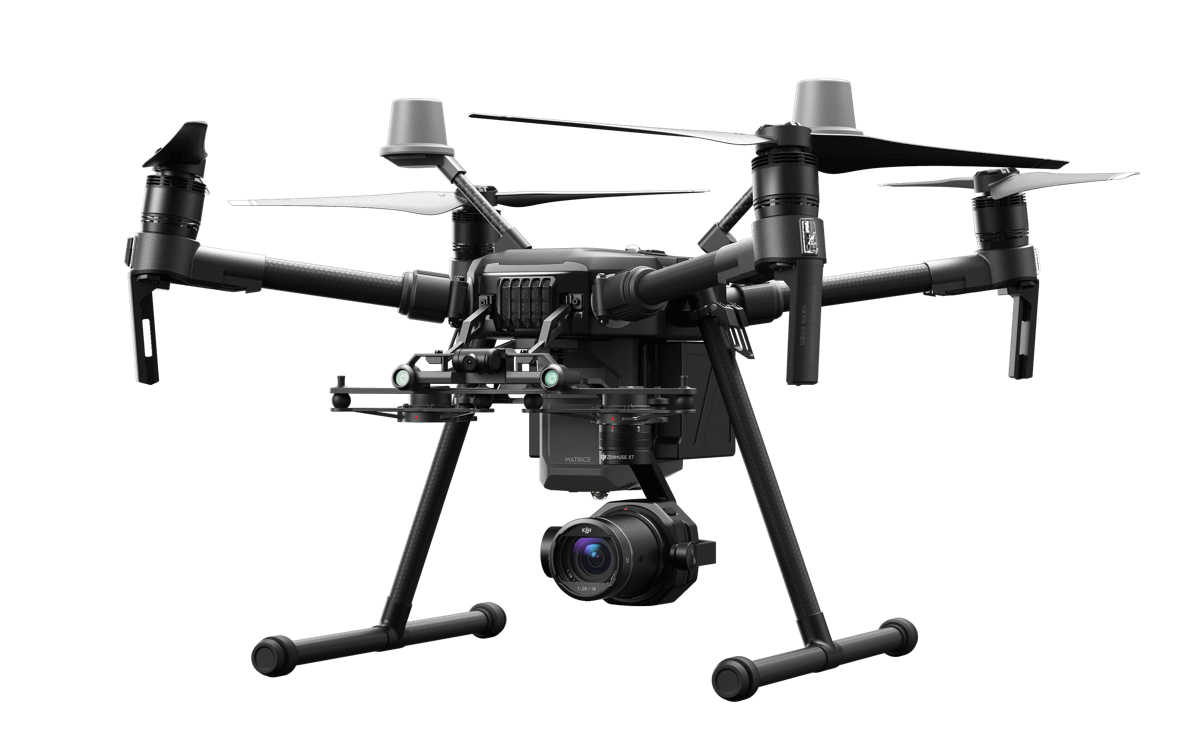
\includegraphics[width=8cm,height=6cm]{Images/drone.png}
    \caption{DJI Matrice 210 RTK v2, Source: DJI website}
    \label{fig:droneimg}
\end{figure}

The main features of the drone are:
\begin{itemize}
    \item Comes installed with Manifold 2, an enterprise version of NVIDIA Jetson TX2 on-board computer which enables the drone to work as autonomous robot with developed software and applications. Manifold 2 runs on Ubuntu 16.04 operating system.
    \item Supports Robot Operating System (ROS) for using drone in the robotic environments.
    \item On-board SDK and ROS On-board-SDK are the open source developer tools offered by DJI. This reduces the burden of creating base packages to communicate with the hardware and adapting the same to ROS environment.
    \item Drone comes with multiple cameras such as front stereo cameras, downward stereo cameras, First Person View (FPV) camera and a high-end payload camera with gimbal. The payload camera is a Zenmuse X5S that comes with a micro 4/3" sensor supporting eight standard M4/3" lenses ranging from 9 mm-45 mm. For our work, the Olympus M.Zuiko 45mm / 1.8 lens was employed. 
    \item Other sensors like IMU sensor, Infrared sensors and Global Navigation Satellite System (GNSS) which supports GPS, GLONASS, BeiDou and Galileo. 
\end{itemize}

\section{ORB-SLAM3}
\label{sec:techbg:orbslam3}
ORB-SLAM is a Simultaneous Localization and Mapping (SLAM) solution for Monocular, Monocular-Inertial, Stereo, and RGB-D cameras. It can compute the camera keyframe trajectory and a sparse 3D reconstruction of the scene in real time in a wide range of scenarios, from small sequence to a vehicle driving around the few city areas. It comes with a robust and automatic initialization from both planar and non-planar scenes. It can close large loops and conduct global re-localization from a wide range of baselines in real time. ORB-SLAM project started off with Monocular Visual SLAM in their first library ORB-SLAM \cite{murAcceptedTRO2015}. They released the next version called ORB-SLAM2 \cite{murORB2} which features Stereo and RGB-D camera based SLAM solution. \\

At present, the ORB-SLAM3 \cite{ORBSLAM3_2020} is the cutting edge release from the same project which features Visual Inertial SLAM i.e Monocular Inertial SLAM solution. ORB-SLAM3 as whole includes all the prior features from ORB-SLAM and ORB-SLAM2. They also claim in their paper \cite{ORBSLAM3_2020} that ORB-SLAM3 is the first system capable of performing visual, visual-inertial and multi-map SLAM with monocular, stereo and RGB-D cameras and supports pin-hole as well as fish-eye models.
This approach is more robust and two to five times accurate than previous approaches. It is also an open-source library, free for all to use for research and development purposes. \\

There are several other Visual SLAM and VI-SLAM libraries as open-source tools such as VINS-Mono \cite{Geneva2020ICRA} and \texttt{open\_vins} \cite{qin2017vins} but for our work we consider ORB-SLAM3 and try to work through it to get the results.

\section{GeographicLib}
\label{sec:techbg:geographiclib}
GeographicLib \cite{GeographicLib} is a simple C++ libray which provides methods for Geodesic conversions, Geoid modeling and gravity and magnetic field calculations. The main highlights of the library is that it supports conversion between Universal Transverse Mercator (UTM), Universal Polar Stereographic (UPS), WGS84 system, Earth Centric Earth Fixed (ECEF) and local coordinate systems like ENU and NED. This library reduces the overhead of developing custom methods to compute the conversion. In this internship, this library is employed in the second latter part of work where we develop a geo-referening node parallel to ORB-SLAM3 custom node. The following methods are used in the development of the node-
\begin{itemize}
    \item WGS84 to ECEF conversion.
    \item WGS84 to ENU conversion.
    \item Creating WGS84 earth model for the reference used in conversions. 
\end{itemize}

\section{Kalibr}
\label{sec:techbg:kalibr}
Kalibr \cite{Kalibr} is a conglomeration of tools for different kinds that help in solving calibration problems. This tool was created by referring to many papers but the main work published is \cite{7487628}. The toolbox offers the following tools-
\begin{itemize}
    \item Multiple camera calibration.
    \item Camera-IMU calibration.
    \item Rolling Shutter Camera calibration.
    \item Other co-supporting tools.
\end{itemize}

In our work, Camera-IMU calibration tool \cite{6696514}\cite{6225005} is used to generate transformation matrix between camera and IMU sensor. 

\vspace{1cm}
Further, we move to new chapter which will explain the initial setup, installation and architecture for the development.   
\chapter{Concept}
\label{ch:concept}
The main aim of the task is to setup the drone to work in the environment of Robot Operating System (ROS) for the purpose of custom ORBSLAM3 package development which estimates Camera Pose and Keyframe trajectory in any given coordinate system. Orbslam3 or Orbslam in general computes and detects key points on the image frame using ORB features and estimates camera pose of the current frame in real-time. Camera pose data consists of the position of the camera center in the orbslam coordinate system and orientation of the camera with respect to the orbslam coordinate system. These results helps in 3D reconstruction or scene reconstruction. The camera poses and trajectory can be scaled to any coordinate system of our choice namely ENU or ECEF for a global view. \\

Previously, every other experiment on the topic of Visual SLAM or VI-SLAM were processed offline using recorded data. This approach takes a step ahead to run the SLAM systems while the drone is flying and get the live camera poses and keyframe trajectory. The usage of ROS bolsters our approach by providing real-time data publishing-subscribing platform on par for an online processing scheme. Even though Orbslam3 native library supports Visual SLAM and VI-SLAM without ROS environment, developing a custom package using ROS and SLAM systems provided by the native library creates a flexible support for the usage of APIs. \\

Initial goal was to run the Visual SLAM and VI-SLAM on the drone and test the ORBSLAM3's out-of-box functionalities and to understand the resources which paves way to the planning for the development course. Moreover, to achieve this, it needs prerequisites such as setting up the drone's on-board computer (Manifold 2) by installing SDK and ROS SDK for our needs. Moving on, as sections of this chapter, we shall discuss and explain different prerequisite tasks that were carried out to support the main goal.

\section{Initial Architecture}
\label{sec:concept:archi}
Architecture, as shown in the Fig Fig \ref{fig:architecture}, of any major task plays an important role to have a basic understanding of the system development and to list out sub sections in the development phase of a package. The architecture described below is architecture of the ROS package named as \texttt{vid\_orbslam3}. The main node in the package subscribes to image topic in our case named as  \texttt{/dji\_osdk\_ros/main\_camera\_images} published by the drone's on-board computer for the purpose of Visual SLAM and subscribes to both image topic and IMU topic i.e \texttt{/dji\_osdk\_ros/imu} for the purpose of VI-SLAM. Therefore, these two ROS topics published by bringing up the drone is used as inputs to our custom orbslam3 node. \texttt{vid\_orbslam3} node make use of orbslam3 library classes and methods to setup a SLAM mechanism in the ROS environment. Additional features such as saving the camera intrinsic parameters, Hamilton Quaternion Multiplier method and saving the Keyframe trajectory data into a file are developed into the \texttt{vid\_orbslam3} package. \\

We finally expect two fruitful outputs namely Camera Poses and Keyframe trajectory. These two results are to be published as Keyframe Graph as a custom posearray topic. This is the basic architecture planned for the initial phase of the development. After looking at the results, other parts of the architecture are to be added and facilitated. 

\begin{figure}
    \centering
    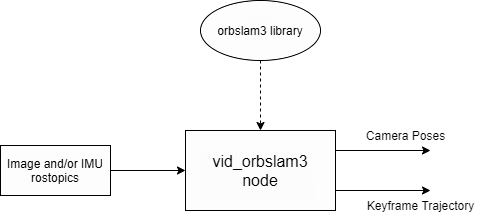
\includegraphics[height=5cm, width=9cm]{Images/archi.png}
    \caption{Architecture}
    \label{fig:architecture}
\end{figure}

\section{Setting up manifold 2 on-board computer}
\label{sec:concept:settingupmanifold}
The on-board computer supported by the DJI Matrice 210 series drone is Manifold 2. As discussed in technical background chapter, Manifold 2 runs on Ubuntu 16.04. Therefore, this computer runs as similar to as any other ubuntu system. This eases out the installation process of tools and libraries for the development. To access the data out of the drone peripherals and sensors for the purpose of processing, a SDK is needed. DJI developer community provides DJI onboard SDK \cite{DJI_OSDK} and DJI Onboard ROS SDK \cite{DJI_OSDK_ROS}. \\

At first, DJI Onboard SDK was installed onto the Manifold 2 using DJI's official documentation. Tests such as gimbal control, camera selection were performed using example code provided by the SDK package. This SDK installation is prerequisite for installing Onboard ROS SDK. As the task needs ROS environment development, ROS Kinetic Kame distribution was chosen to be installed on the Manifold 2 as Ubuntu 16.04 supports only Kinetic Kame. Following the official ROS documentation, ROS was installed and a separate work space for the development was created. It was also noted that, OpenCV 3.3.1-dev version was installed along with ROS. The OpenCV version installed on the system might affect or impact on the development of the \texttt{vid\_orbslam3} package using native orbslam3 library. \\

Further, Onboard ROS SDK was installed using standard ROS package installation into the ROS work space. The following commands were used compile the Onboard ROS SDK into the ROS work space:

\begin{lstlisting}[language=bash, basicstyle=\small]
$ cd catkin_ws/src
$ git clone https://github.com/dji-sdk/Onboard-SDK-ROS.git
$ cd ..
$ catkin_make 
\end{lstlisting}

Once the compilation ends, the onboard SDK for ROS is ready for usage. The ROS SDK comes with a launch file under launch folder which should be used to bring up the drone for ROS functionalities. It helps us launch the vehicle node that brings up the drone to ROS environment and publishes the peripheral and sensor data as ROS topics. These topics can be used by other nodes to their extent by subscription. This launch file is named as \texttt{dji\_vehicle\_node.launch} and contains few arguments related to user details. These details are generated when the drone is registered on the official portal for development purposes. A UserConfig.txt file is generated when the DJI Onboard SDK was installed. Fill in information available on UserConfig text file as it is into the argument fields inside the launch file. Without this step, drone cannot be made functional with the launch file. The vehicle node can be launched using the following commands:

\begin{lstlisting}[language=bash, basicstyle=\small]
$ roscore
$ roslaunch dji_osdk_ros dji_vehicle_node.launch
\end{lstlisting} 

ROS topics are published under the tag \texttt{/dji\_osdk\_ros/t\_name} and topics include main camera images, FPV images, left and right stereo images, IMU, GPS, gimbal angle and other useful topics.

\subsection*{Initiate Main Camera Images publishing}
\label{subsec:settingupmanifold:inititecamera}
With DJI ROS SDK, the camera topics are available as ROS topics once the vehicle node is brought up. But the data is not available until the camera service is called manually using rosservice call. This is done to reduce the overhead on the vehicle node to omit the camera topics which are not needed. Camera service call is available for all the cameras namely main camera, FPV camera and stereo cameras. Therefore, a shell script was written to automate the bringing up of the drone and select the required camera topics to publish.
Since, the task was mainly using the main camera, \texttt{/setup\_camera\_stream} service was available and rosservice was called with suitable inputs to trigger the publish.

\section{Installing ORBSLAM3 Library}
\label{sec:concept:orbslam3lib}
As discussed earlier, ORBSLAM3 library provides classes and methods to perform Visual SLAM, VI-SLAM and multi-map SLAM. Based on the official documentation, ORBSLAM3 library was tested on Ubuntu 16.04 and 18.04. This library requires C++11 compiler, Pangolin tool for visualization purposes, atleast OpenCV 3.0 and Eigen library 3.1.0 version or higher. ROS installation is optional for compiling the ORBSLAM3, but as per the task we have installed ROS as well. ORBSLAM3 was compiled following the instructions given in the official documentation. \\

Initially it was compiled and tested on a local computer having Ubuntu 18.04 and other required dependencies before it was compiled on the Manifold 2. Using the example code and EuRoC data set \cite{Burri25012016} (V1\_02\_medium.bag), ORBSLAM3 Monocular Visual SLAM and VI-SLAM were tested for better understanding of the library offered. Further, the same procedure was followed to compile the library on the Manifold 2. 

\vspace{1cm}
In the next chapter, we shall discuss on the implementation of the task. This task is divided into two parts. In the first part, the development of the vid\_orbslam3 package for Visual SLAM and VI-SLAM are explained, discussion on IMU sensor calibration and computing body-camera transformation matrix, discussion on failure of VI-SLAM on our setup and observations made on other SLAM systems such as Vins-Mono \cite{qin2017vins} and open\_vins \cite{Geneva2020ICRA}.

\chapter{Implementation-1}
\label{ch:implementation}
\section*{Part 1}
\label{sec:implemenation:part1}
\section{Camera Calibration}
\label{sec:camcalib}
Cameras in real life introduce significant amount of distortion to the images due to internal or external influences. There are 2 types of distortions – Tangential distortion and Radial distortion. Radial distortion makes the straight lines in the image to be curved. Tangential distortion takes place when the lens of the camera is not aligned parallel to the sensor plane. Due to this the image appears to be closer than in reality. To overcome these errors, camera calibration is done to obtain the distortion coefficients, camera matrix and other necessary camera data rectify the distorted image.\\

ORBSLAM3 takes in a yaml settings file that specifies camera intrinsic parameters, distortion parameters and ORB parameters. We can extract intrinsic and distortion parameters from camera calibration process.
ROS contains out-of-box camera calibrator python script which allows the user to calibrate the camera.  The below command is use to carry out the calibration process in ROS.
\begin{lstlisting}[language=bash, basicstyle=\small]
$ roscore
$ rosrun camera_calibration cameracalibrator.py  
- -size 8x6 - -square 0.075 image:=/dji_osdk_ros/main_camera_images  camera:=/camera
\end{lstlisting} 

So obtained parameters from this calibration was updated into the settings file for the ORBSLAM3.

\section{vid\_orbslam3 package for Visual SLAM}
\label{sec:initialpackagevslam}
The package vid\_orbslam3 was developed as a ROS package to create a node that subscribes to a camera image topic and perform monocular visual SLAM for each image frame. ORBSLAM3 library provides definite methods which can be used to initiate and perform monocular SLAM through our node. The ORBSLAM system object is instantiated as a monocular functioning entity. Since ORBSLAM3 uses pangolin for the visualization, it is impractical to use visualization on a headless Manifold 2. However, the display of the visualization can be switched on/off with our node for specific usage if a monitor is connected for debugging. Some utilities that were developed as part of this task are as follows -
\begin{itemize}
    \item Method that stores the camera intrinsic and distortion parameters for usage.
    \item Method that performs Hamilton product between 2 quaternions.
\end{itemize}
The node takes in vocabulary file and settings file as input that contributes information for keypoint detection and pose estimation. ORBSLAM3 system class provides method named as \emph{System::TrackMonocular} for performing monocular SLAM tracking. For every image frame, the above method returns a camera pose matrix \((^wT_c)\) in orbslam coordinate system. The entity or object created before is used for the invocation of the above tracking method. The camera poses returned are transformed into ROS coordinate system with rotation matrix \((^{ros}R_{orb})\) and published as a pose topic. Alternatively, the pose can also be broadcast as a transform or TF.

\begin{align}
   ^{ros}R_{orb} =
   \begin{bmatrix}
   0 & 0 & 1\\
  -1 & 0 & 0\\
   0 & -1 & 0
   \end{bmatrix}
\end{align}

The node was tested using a pre-recorded rosbag recorded using the drone and we were able to visualize the pose on Rviz. Nevertheless, the results are not acceptable until tested in real-time. For this the drone has to be made as a slave and a local PC as master for the real-time camera pose visualization. In the next section, a brief explanation is given about the ROS master-slave setup.

\section{ROS master-slave setup}
\label{sec:masterslavesetup}
In real-time, visualization of camera pose plays important role for UAV based SLAM implementations. ROS solves the problem of remote visualization with it's master-slave functionality. This setup requires both the drone and the local PC to be connected to same local network. Run the following linux commands in the working terminal for both master (loacl PC) and slave (Manifold 2)-\\
\\
Master side:
\begin{lstlisting}[language=bash, basicstyle=\small]
$ export ROS_MASTER_URI=http://<IP-addr-of-master>:11311/
$ export ROS_HOSTNAME=<IP-addr-of-master>
\end{lstlisting}
Slave side:
\begin{lstlisting}[language=bash, basicstyle=\small]
$ export ROS_MASTER_URI=http://<IP-addr-of-master>:11311/
$ export ROS_HOSTNAME=<IP-addr-of-slave>
\end{lstlisting}

If multiple terminals are used for execution, for uniformity, add these lines into respective .bashrc files. After this, both the systems are ready for master-slave functionality.

\section{Drone flight and vid\_orbslam3 node}
\label{sec:droneflight}
The drone and the local system was setup as explained before and  vid\_orbslam3 node was launched using a ros launch file. As expected, we obtained real-time camera poses through the published rostopics. The visualization was made using Rviz tool on the local PC. But it was observed that monocular SLAM resets the map and tracking when the vehicle moves too quickly. This affects the motion of the camera and hence will not allow monocular SLAM system to detect keypoints in turn punishes the pose estimation process. A similar observation in an article \cite{Luo2020} was reported for poor feature point extraction and system tracking failure due to motion blur caused by quick camera rotation or movements at large angles.

\subsection*{Need for Visual Inertial SLAM}
Interestingly, it was also found that Visual SLAM has scale ambiguity and is suitable for indoor environments. To overcome this, stereo cameras are used for the correction. For catering single camera setup, IMU fusion with the camera resolves the scale ambiguity. This results in Visual Inertial SLAM. ORBSLAM3 offers VI-SLAM as a new add-on from it's previous release ORBSLAM2. Hence, VI-SLAM is suitable for both indoor and outdoor environments. IMU measurements can provide quick velocity and absolute scale information ramping up the estimation process as explained in \cite{7487266}.

\section{IMU calibration and T\textsubscript{bc} estimation}
\label{sec:imucalib}
ORBSLAM3 library offers Visual Inertial SLAM as mentioned in the previous section \ref{sec:droneflight}. The SLAM settings file for VI-SLAM extends Visual SLAM settings file and requires IMU intrinsic parameters and extrinsic parameters or transformation matrix from body to camera \((T_{bc})\) as additional information. Camera pose estimation in case of VI-SLAM takes IMU measurements into consideration. A pose estimation may fail or can have induced error if the intrinsic parameters are not accurate. This process is very much sensitive on IMU intrinsic parameters which boils down to the order of 10\textsuperscript{-4} or sometimes even lower depending on the quality of the IMU sensor.\\

IMU intrinsic parameters consists of 2 values: Additive White Noise (AWN) and Bias also termed as random walk. These two parameters are applicable for both accelerometer and Gyroscope of the IMU module. Therefore, a set of IMU intrinsic parameters has 4 values to be measured. The below equation is the IMU noise model presented by the Kalibr \cite{Kalibr}.

\begin{equation}
    \Tilde{\omega}(t) = \omega(t) + b(t) + n(t) 
\end{equation}

where $\Tilde{\omega}$(t) denotes angular rate measurement, $\omega$(t) denotes actual angular rate, b(t) is random walk or bias and n(t) is additive white noise of one single axis of gyroscope. This equation applies to other axes as well as for the accelerometer. \\

Our drone is considered as an autonomous aerial robot whose motion and attitude are agile. Some of the VI-SLAM implementations provide online IMU intrinsic parameter calculation. But findings presented by Yang et al. \cite{Yang2020} explains the observability of all the 6 axes of IMU sensor while calculating the intrinsic parameters online and why offline calibration is still effective in the case of autonomous robot like environment.

\subsection*{Calibrating IMU intrinsic parameters}
To calculate the intrinsic parameters, additive white noise and random walk, a 2-hour rosbag was recorded containing IMU ros topic /dji\_osdk\_ros/imu from the drone. In the DJI Matrice 210 RTK v2, the IMU sensor is set to publish fused data at 400 Hz. Good results are achieved when calibrated using raw data. Therefore, we used the drone's pilot to change the IMU sensor publish mode to raw data at 400 Hz. 

\begin{figure}[h]
    \centering
    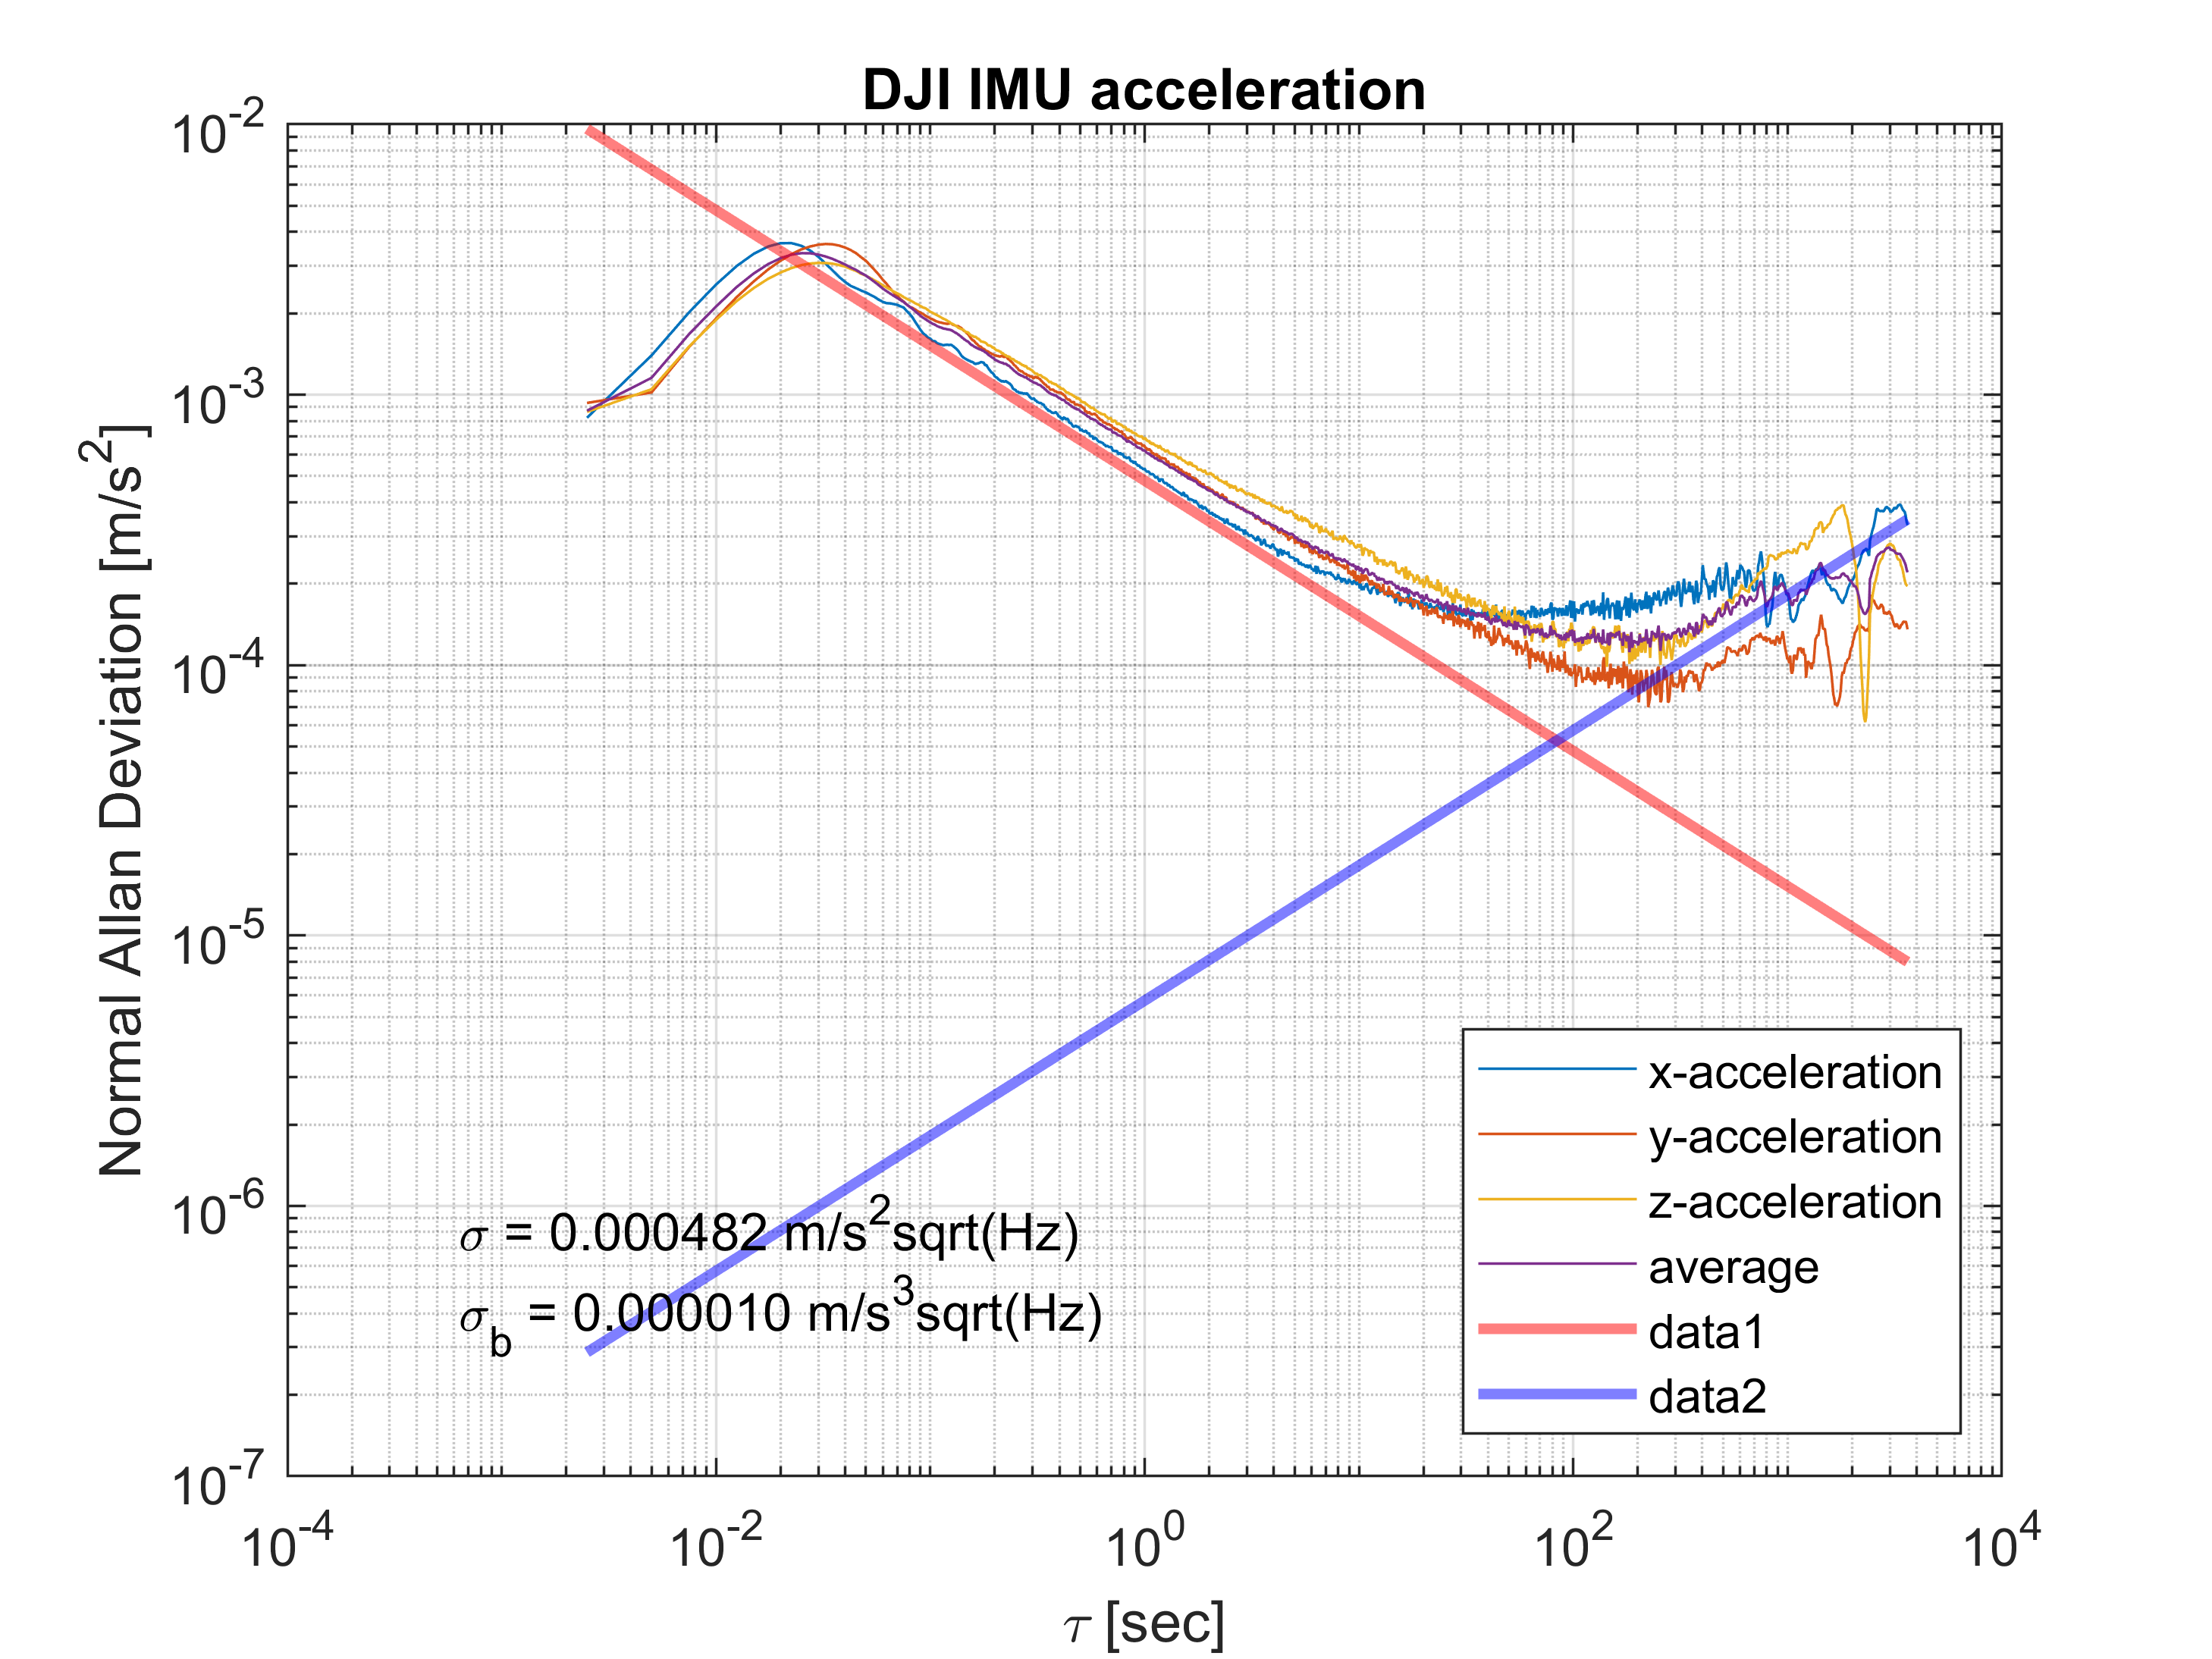
\includegraphics[scale=0.7]{Images/DJI_IMU_accel.png}
    \caption{Allan Deviation plot for Accelerometer}
    \label{fig:accel}
\end{figure}

\begin{figure}[h]
    \centering
    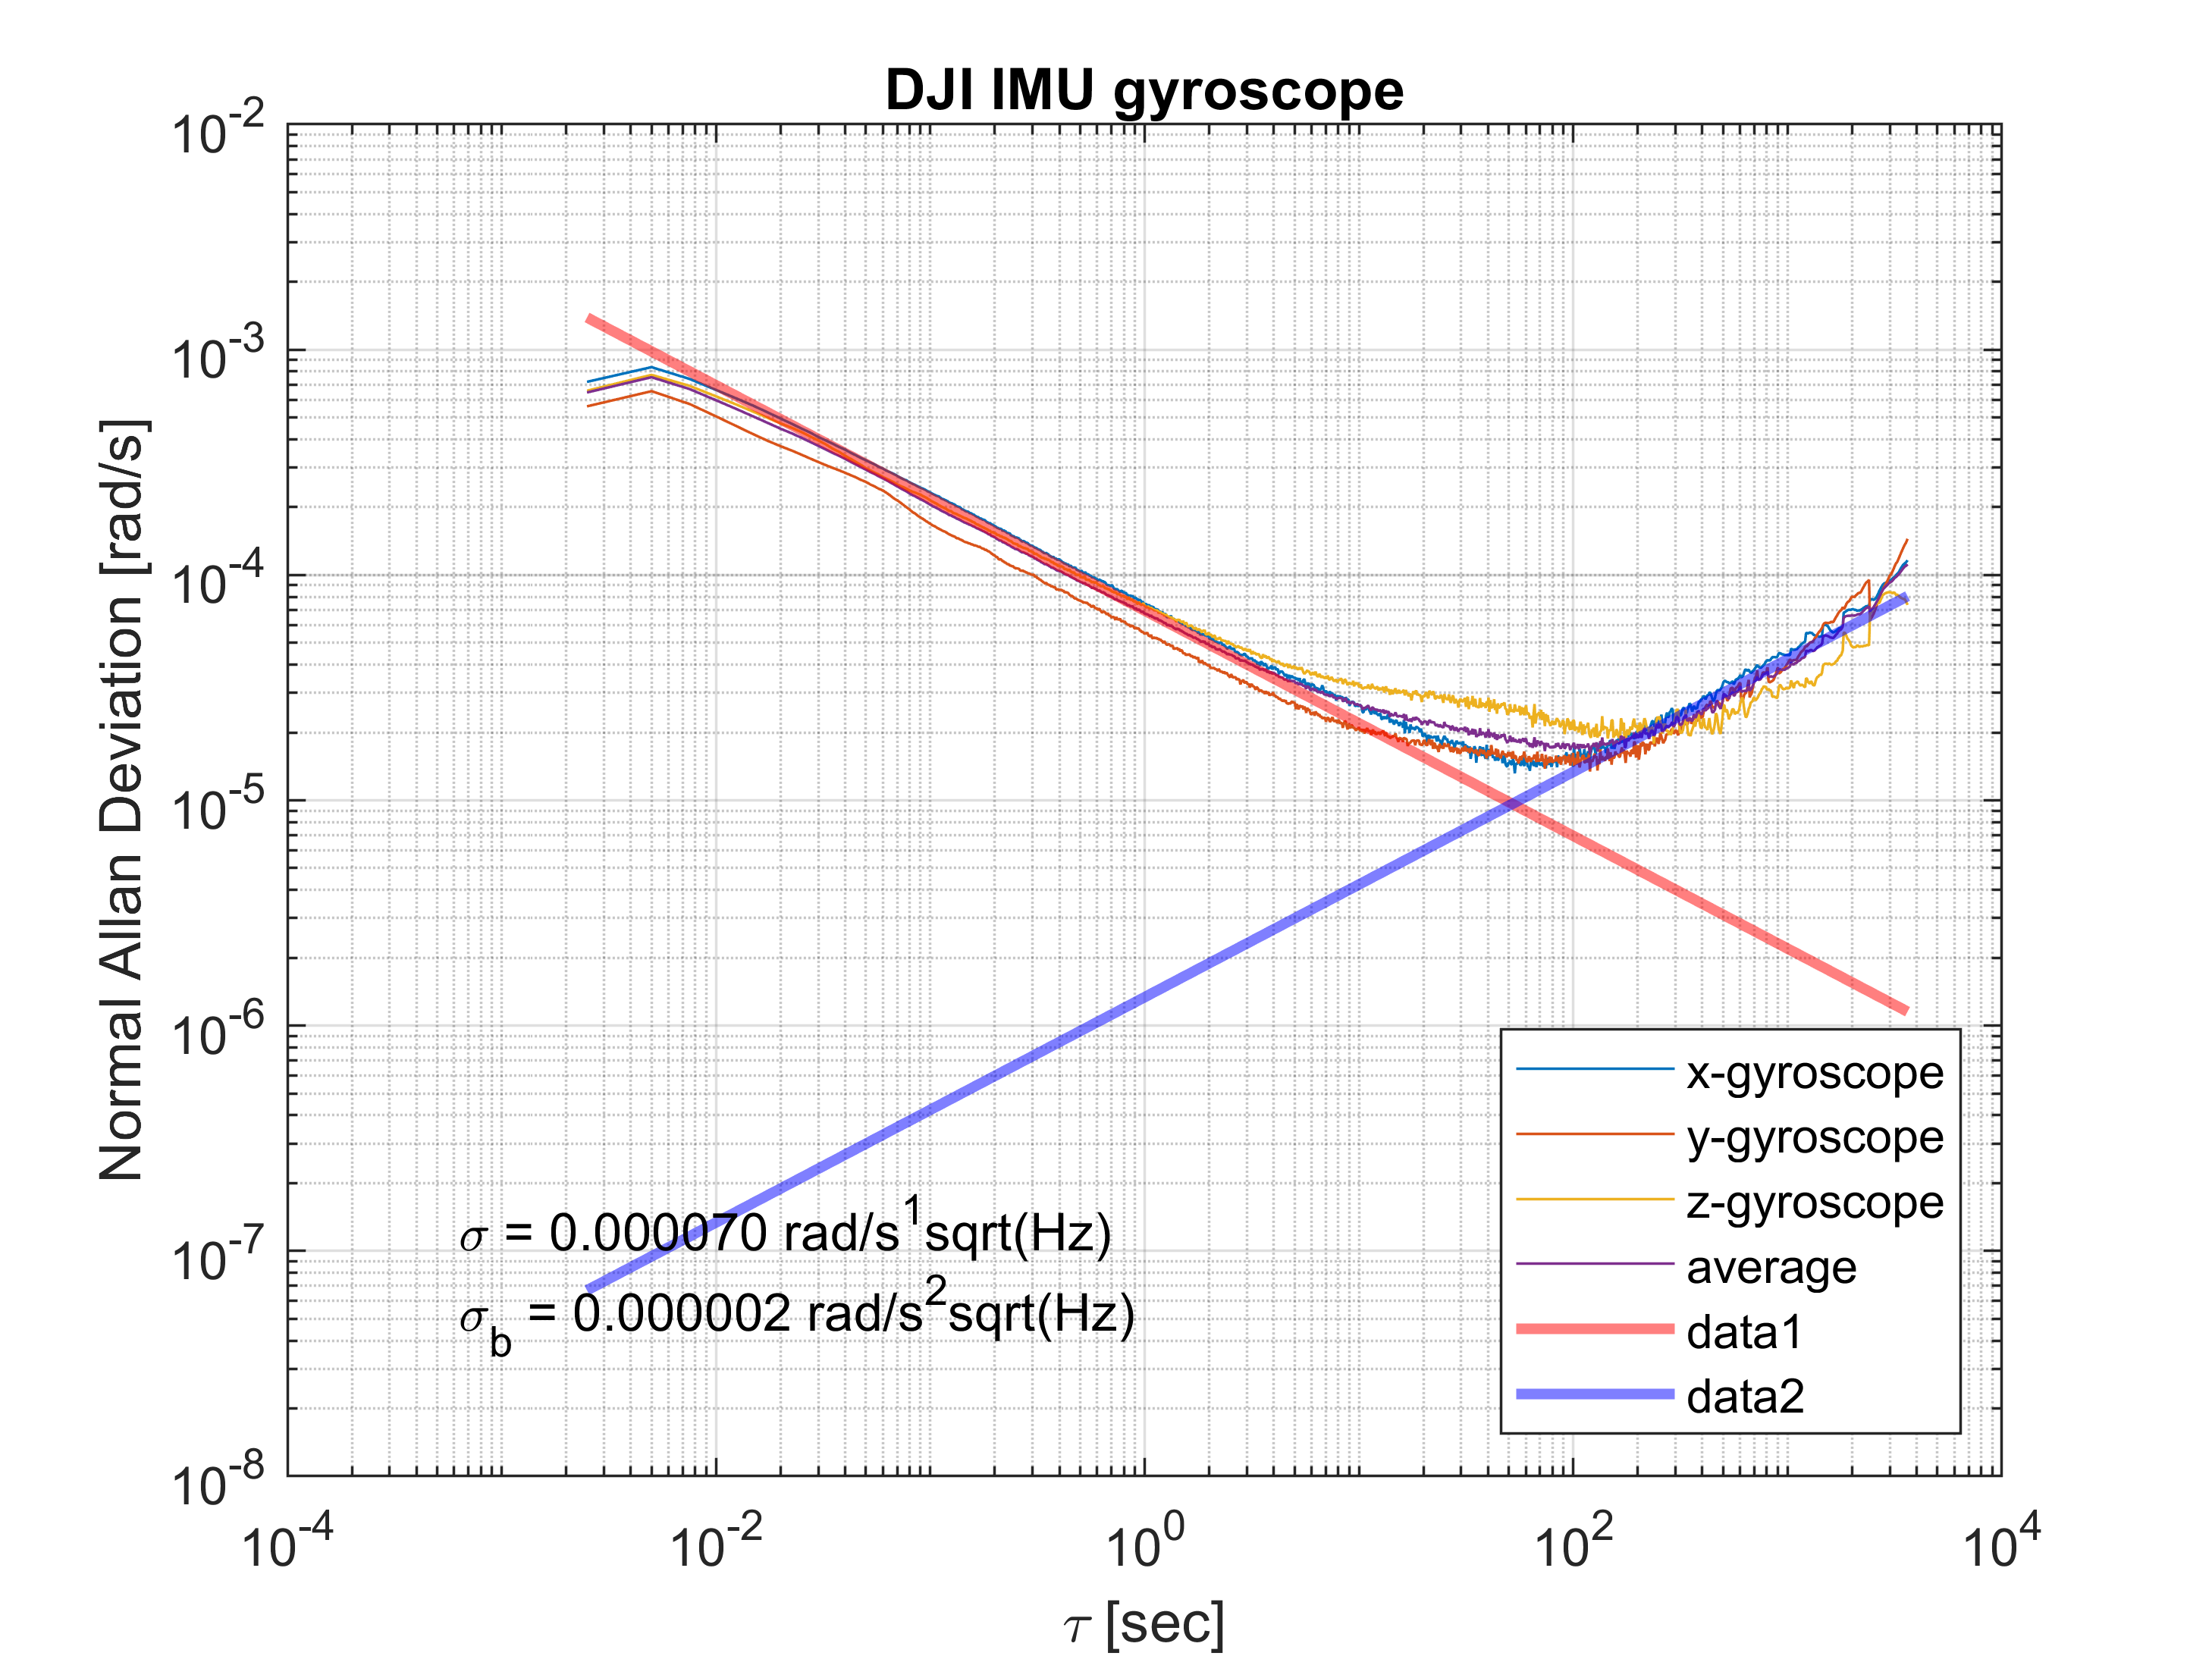
\includegraphics[scale=0.7]{Images/DJI_IMU_gyro.png}
    \caption{Allan Deviation plot for Gyroscope}
    \label{fig:gyro}
\end{figure}

Initially before recording, the drone was rotated, lifted and panned to excite the IMU sensor in all the axes. This helps in stabilizing any excitation error.The drone was also kept on a stationary platform and was undisturbed. Kalibr\_allan tool \cite{kalibrallan} was used for the calibration and the further steps for this process was followed as given in their official documentation.\\

The results obtained from this calibration were as follows:

\begin{itemize}
    \item Additive white noise for accelerometer, $\sigma\textsubscript{n}$ = 0.000482 $m/s\textsuperscript{2} . \sqrt{Hz}$
    \item Random walk or bias for accelerometer,  $\sigma\textsubscript{b}$ = 0.000010 $m/s\textsuperscript{3} . \sqrt{Hz}$
    \item Additive white noise for gyroscope, $\sigma\textsubscript{n}$ = 0.000070 $rad/s . \sqrt{Hz}$
    \item Random walk or bias for gyroscope,  $\sigma\textsubscript{b}$ = 0.000002 $rad/s\textsuperscript{2} . \sqrt{Hz}$
\end{itemize}

Also, the allan deviation plot was observed as shown in the Fig \ref{fig:accel} and Fig \ref{fig:gyro}. This process was performed multiple times to obtain the optimum values.

\subsection*{Calculating T\textsubscript{bc} matrix}
To synchronize the camera and body of the drone for the functioning of the VI-SLAM in general, a transformation matrix T\textsubscript{bc} is required by the system to calculate the camera poses. For this we used Kalibr camera-IMU calibration tool \cite{Kalibr}. The tool uses April Grid calibration schematic and a rosbag containing the movement of the drone in all the 6 axes of the IMU sensor with the camera feed. Further, the tool was used according the documentation and was able to generate T\textsubscript{bc} matrix and the value of the same is as follows:

\begin{align}
   T\textsubscript{bc} =
   \begin{bmatrix}
   -0.03292984 & -0.99925777 & -0.01998826 & 0.\\
  -0.06664725 & 0.02215003 & -0.99753071 & 0.\\
   0.99723306 & -0.03151636 & -0.06732718 & 0.\\
   0.     &     0.     &     0.     &     1.
   \end{bmatrix}
\end{align}

Since, the drone's main camera is installed with the gimbal, it was unable to fix the gimbal to single stationary position to record the movement of the drone. The gimbal auto-corrected the orientation of the camera with respect to the movement and rotation. We decided to use the FPV camera and a re-calibration was performed as explained in the Section \ref{sec:camcalib}.\\
\\
Intrinsic parameters and T\textsubscript{bc} values were updated in the settings file for the Visual Inertial SLAM. 

\section{vid\_orbslam3 node for Visual Inertial SLAM}
\label{sec:vidorbslam3VI-SLAM}
The vid\_orbslam3 node implementation from Visual SLAM was modified to work in Visual Inertial SLAM mode or in ORBSLAM3 terminologies, monocular-inertial mode. In this case, the node had to subscribe to IMU topic (/dji\_osdk\_ros/imu) from the drone. The node was accordingly developed to subscribe to both the topics at the same time and was made sure the camera frames and the IMU data were synchronized. The node was executed similar to Visual SLAM implementation mentioned in section \ref{sec:droneflight}. 

\subsection*{Observation}
Generally, the orbslam3 system takes a few frames to initialize itself and sets the first frame of the detection of key points as initial frame or the reference frame for the SLAM system. Every camera pose is determined with respect this initial frame. Interestingly, after every 2 frames the map was reset and the system was re-initialized for VI-SLAM. The main library code was debugged to find out what was the hindrance and reason for the map reset. It was found that there were not enough key points to consider the frame for the key frame list. Looking at this, it was evident that the keyframe graph is updated and a trajectory can be visualized only for a continuous tracking scenario.

\subsection*{Reasons for failure}
\label{subsec:reasonforfailure}
The above observations were finely investigated to find the reason for the failure of VI-SLAM of ORBSLAM3 on our drone. After trying multiple attempts of re-calibration and re-calculation of intrinsic and extrinsic parameters, the map reset was evident in all the attempts. On later stages of this investigation, one of the reasons for failure was found: ORBSLAM3 does not support rolling shutter cameras. Rolling shutter effects play a vital role in false point correspondences and key point extraction. Also, rolling shutter frame has a read out delay of in milli-seconds with at least 1/FPS ms. \\

Unfortunately, the main camera and the FPV camera on our drone DJI Matrice 210 RTK are rolling shutter cameras. It is convincing that, modeling the rolling shutter cameras for Visual SLAM or VI-SLAM is quite a task and even though when achieved the results are not satisfactory as compared to global shutter cameras. It was a good insight for us to plan the next stages of the task.

\newpage

\section{Testing other SLAM systems}
\label{sec:otherslamsystems}
Another attempt to implement VI-SLAM on the drone was made by employing other software implementations in the field of VI-SLAM. VINS-Mono \cite{qin2017vins} and open\_vins \cite{Geneva2020ICRA} were chosen to be tested on our platform with previously deduced IMU parameters and camera setup. Apparently, VINS-Mono supports rolling shutter cameras. But the performance analysis index using rolling shutter camera with VINS-Mono was rated the lowest among the other combinations of Global shutter camera and low to high end IMU sensors in their documentation.\\

VINS-Mono was installed on the local PC following the official documentation. A rosbag was recorded for the purpose of testing the VINS-Mono. The settings file for the VINS-Mono was similar to that of ORBSLAM3 and the corresponding fields in the settings file were updated with our findings from calibration. The example code was available for ROS environments and the VINS-Mono was tested with the recorded rosbag. Repeatedly, the Visual Inertial SLAM was failing here as well. VINS-Mono also considered the camera-IMU delay (t\textsubscript{r}) as an input in the settings file. Our calibration had an expected low delay time. For unknown reasons, the system was failing to track the key points after a couple of frames similar to ORBSLAM3.\\

Moving on, open\_vins was considered and installed on the same local PC following the official documentation. The open\_vins implementation does not explicitly support rolling shutter cameras but in the developer community there were a few attempts made to use rolling shutter camera for VI-SLAM. We attempted to perform VI-SLAM using open\_vins with our setup. Besides a lot trials in finding the right threshold to excite IMU at the drone's lift off to trigger the SLAM action to start (required by the open\_vins node), the position trajectory was drifting far away after a few seconds with drone being stationary held. From this observation, we were skeptical about the IMU intrinsic parameters because our values were really low. This results in highly sensitive sensor response while calculating displacement of the vehicle. A small movement of the drone would ramp up a higher response creating a huge drift in position trajectory and visualization. Also, in the settings file of the open\_vins for VI-SLAM, it was possible to specify the pixel noise to compensate the generic rolling shutter effect. We increased the pixel noise 5 to 10 times that of the standard value. Using this when tested, for some time the trajectory was close enough to expected results but down the line when there was a rapid movement of the vehicle, due to motion blur and highly sensitive IMU response would cause the drift. \\

Therefore, I would like to propose a conjecture from all the attempts made and observations analyzed: \textbf{Visual Inertial SLAM is not suitable for a setup whose camera is mounted on the gimbal with rolling shutter}. Visual Inertial SLAM needs a good IMU calibration with stable IMU response. Very low or very high response would lead to failure of accurate IMU calibration in turn leads to the failure of the Visual Inertial SLAM on autonomous aerial vehicles or drones which are bound to agility and undergo external influences affecting the movement of the vehicle. This conjecture is not perfect but sets a baseline for the future developments in this area. A rolling shutter model for VI-SLAM can be developed to handle all the failures as observed by our attempts. Visual Inertial SLAM is a good field to explore and has room for interesting results to come.

\subsubsection*{New attempt planned for the task}
To continue with Camera pose and keyframe trajectory estimation, we planned to drop the Visual Inertial SLAM on our setup. As the Visual SLAM was reasonable enough and tested to get the camera poses, it was decided to use the GPS data from the drone with Visual SLAM to achieve the task goals. Next sections in this report is designated as Part 2 of the task. The know-how and implementation of Visual SLAM with GPS data will be discussed in the further sections.


\chapter{Implementation-2}
\label{ch:implementation2}
\section*{Part 2}
\label{sec:part2}
In the part 1, we tried implementing vid\_orbslam3 node to perform VI-SLAM on our drone setup. As explained in the previous chapter, the attempts failed to give results for various reasons. To continue the pose and keyframe trajectory estimation, we planned to use GPS data with Visual SLAM and adapt it to a local coordinate system of choice. This chapter explains the method, architecture, challenges, observations and results of the implementation.

\section{Architecture}
\label{sec:architecture2}
The architecture is a continuation of the previous architecture from Section \ref{fig:architecture}. The gps\_process node is a stand-alone node which runs on a local PC subscribing to the keyframe graph topic from the vid\_orbslam3 node and the GPS topic from the drone. The following block diagram depicts the architecture of the implementation.

\begin{figure}[h]
    \centering
    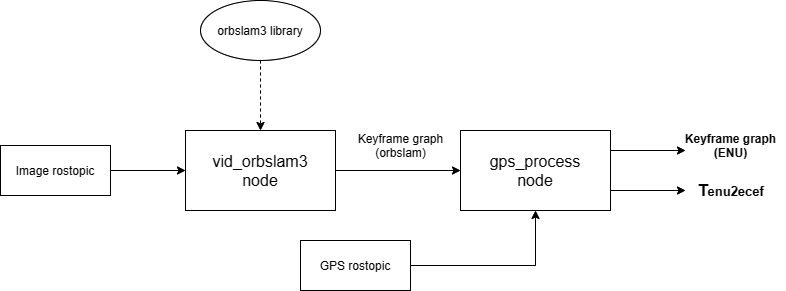
\includegraphics[height=4.5cm, width=10cm]{Images/archi2.png}
    \caption{Architecture for Visual Inertial SLAM with GPS}
    \label{fig:archi2blk}
\end{figure}

A suitable method is used to estimate the keyframe graph in East-North-Up (ENU) system and a static transform is published between ENU and Earth Centric Earth Fixed (ECEF) system for external tool or software for visualization. There are other approaches to fuse gps data into the bundle adjustment of the SLAM system, but it would become a separate project to develop. Finally it was decided to move ahead with our architecture.

\section{Processing Keyframe graph}
\label{sec:processingKFgraph}
The vid\_orbslam3 node was reverted back to work as Visual SLAM mode. To transform the keyframe graph generated by ORBSLAM3 to ENU system, the whole set of keyframe list had to be published as and when a new keyframe is added to the list. The native ORBSLAM3 library has an entity called Atlas that stores all the keyframes at the current instance. When loop closure occurs or redundant frames are removed, Atlas updates itself with a freshly updated keyframe list. We make use of this in our node by adding a new method to the native library. The method is called \emph{System::getAtlas} and it returns pointer to the current Atlas. We recomplied the library and invoked this method in the vid\_orbslam3 node.\\

For every image frame that is subscribed, a fresh list of keyframe graph is updated in vid\_orbslam3 node. For every new keyframe graph obtained it is then published as a rostopic named as /KeyframeGraphSLAM. This topic is of the message type vid\_orbslam3::KeyframeGraph, which is a custom rosmessage that was that was created by us to hold all the current keyframes in an array.\\

Now moving on, we started developing gps\_process node inside our development package. The gps\_process node needs two inputs to process: /KeyframeGraphSLAM, which gives the whole KeyframeGraph at the current instance and the GPS topic /dji\_osdk\_ros/gps, which gives current GPS location of the drone in WGS84 system. Using these two, the whole KeyframeGraph in SLAM co-ordinate system can be converted into East-North-Up (ENU) co-ordinate system. In the further sections we shall explain how the transformation is performed to achieve the task.

\section{Approach to estimate T\textsubscript{slam2enu}}
\label{sec:approachTslam2enu}
The gps\_process node subscribes to keyframe graph topic and gps topic for the estimation purpose. The lift off of the drone is set as the initial coordinate for the purpose of ENU reference. All the gps messages are stored in a list for gps stamping the keyframe. The first step in this approach is to gps stamp every frame in the keyframe graph. Every keyframe in the graph is sorted using the timestamp of the gps message. Since there might be a slight delay in milli-seconds between the KeyframeGraph topic and gps topic, a time difference of less than 2 ms is allowed. By doing this, all the keyframes in the KF graph are tagged with respective gps location in WGS84 format and ENU format. To convert gps location to ENU format, we used GeographicLib \cite{GeographicLib} which offers WGS84 to ENU and WGS84 to ECEF conversions. These tagged keyframes are stored into a list with elements formated as a custom data structure containing pose, gps location and ENU point information.\\

\begin{lstlisting}[language=bash, basicstyle=\small]
struct GPSKeyframe {
 tf::Vector3 ENU;  
 sensor_msgs::NavSatFix gpsCoord; 
 vid_orbslam3::KeyframeStamped KF; 
};
\end{lstlisting}

Further, the stored list is iterated over for SLAM positions in keyframes and ENU positions are separated into separate list for the estimation process. The main idea is to obtain a transformation between the SLAM coordinate system and ENU coordinate system. We make use of colmap's \cite{schoenberger2016sfm} similarity transform and a method was developed in gps\_process node to estimate the transformation. The method requires 2 lists with different coordinate systems.For every new callback from the ros node, a new transformation matrix  T\textsubscript{slam2enu} was estimated. Using this, all the keyframes or poses in the stored list was transformed to ENU coordinate system. Further, a posearray was created and published as a topic named /KeyframeGraphENU.\\

Visualization of the above published topic resulted in an oblique trajectory. The drone flew across the area resulting path trajectory plane is parallel to the earth's surface. Theoretically, a similarity transform should correct any such irregularities with the input to a referenced coordinate system. After multiple attempts to correct this, we analysed the input trajectory and tested the same estimation strategy using 2 static data files, one containing SLAM points and corresponding ENU points. 

\section{Observation in static file data analysis}
\label{sec:staticapproach}
The Visual SLAM generated keyframe trajectory and corresponding ENU points were saved into two different files. As observed from the previous section, the keyframe trajectory in ENU was oblique with respect to the surface of the earth. The input trajectory file generated by SLAM system was plotted to check the sanity of the results from ORBSLAM3. The input /KeyframeGraphSLAM to the gps\_process node was itself oblique as shown below.

\begin{figure}[h]
    \centering
    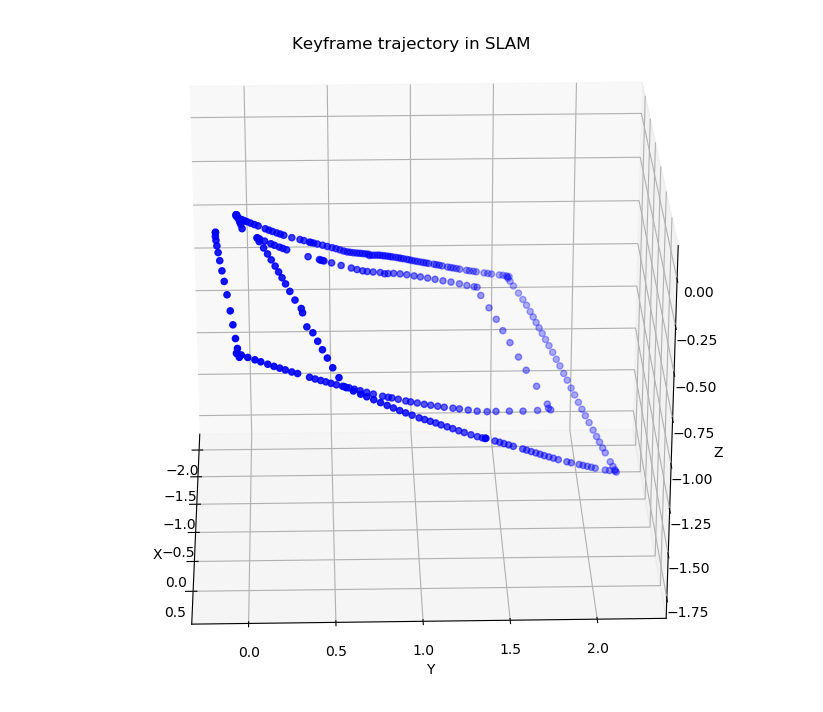
\includegraphics[height=11cm, width=15cm]{Images/KFTrajectoryinSLAMFront.png}
    \caption{Keyframe trajectory in SLAM, Front view}
    \label{fig:kfgraphSLAMfront}
\end{figure}

\begin{figure}[h]
    \centering
    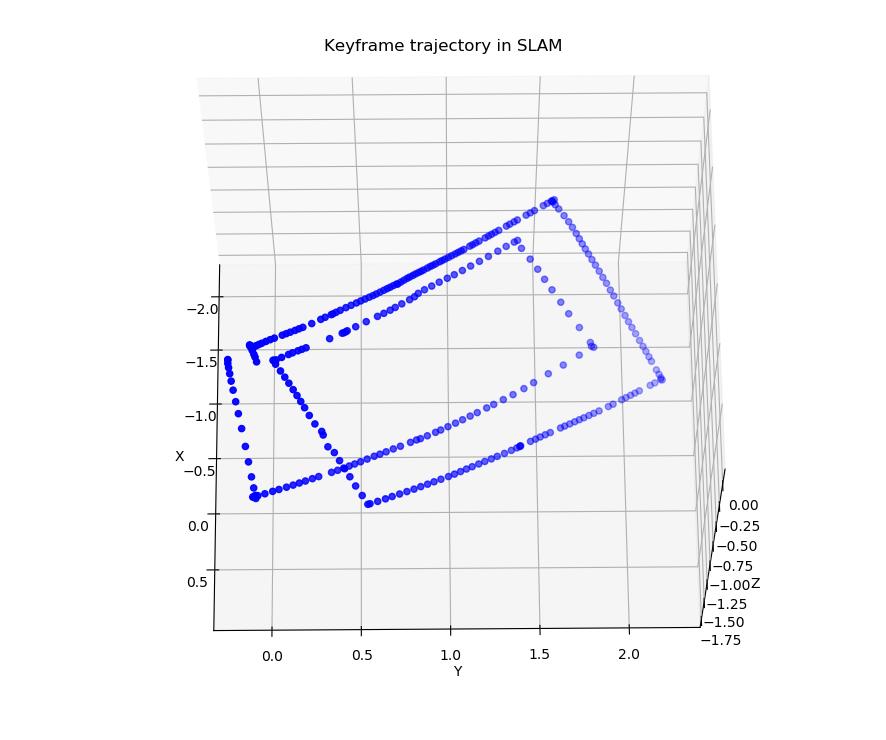
\includegraphics[height=11cm, width=15cm]{Images/KFTrajectorySLAMTop.png}
    \caption{Keyframe trajectory in SLAM, Top view}
    \label{fig:kfgraphSLAMtop}
\end{figure}

From the top view \ref{fig:kfgraphSLAMtop}, it looks to be flat and parallel to the surface. But when observed from the front \ref{fig:kfgraphSLAMfront} we can clearly see the oblique nature of the result. Naturally, when all the current keyframes on list is considered for transformation the resultant in the ENU coordinate system also produces an oblique trajectory curve. This is due to the cumulative effect that Visual SLAM produces from scale ambiguity.\\ 

VI-SLAM would have corrected this obliqueness using it's Inertial sensors (IMU). Since we are not using VI-SLAM, a different approach is needed to tackle overcome this. The measurement scale in the figure \ref{fig:kfgraphSLAMfront} and \ref{fig:kfgraphSLAMtop} are in orbslam3 scale. Usually, this found to be normalized internal SLAM system.

\section{Windowed-selection approach and Robust alignment}
\label{sec:windowandrobust}
Instead of considering all the points in SLAM and ENU system for estimating Transformation matrix, we can construct a window of N where N = 3, 5, 7, 11. This window can slide over both the lists (SLAM points and ENU points), select a group of N elements in the range. For this bunch of N elements are used for estimating transformation matrix. The obtained transformation matrix is used to transform the middle element in the SLAM points window and further the transformed point is added onto the list of transformed points. This process was performed for the complete set of points using both files. When the resultant list of converted points were plotted, we found that the obliqueness of the trajectory was solved. We chose to use window size N = 3. Although, we tried for all the above mentioned sizes.

\begin{figure}[h]
    \centering
    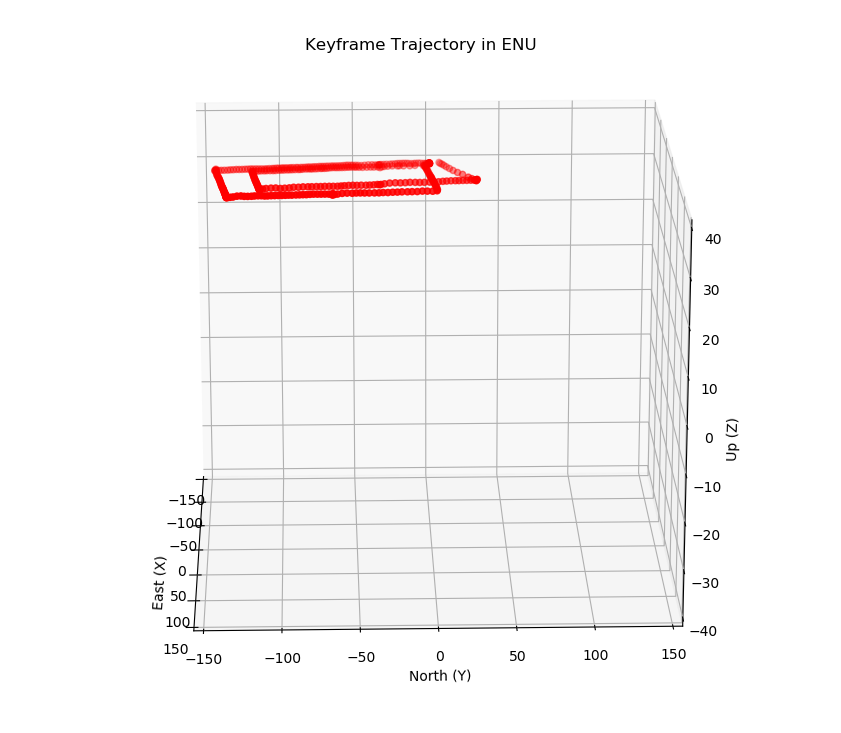
\includegraphics[height=11cm, width=15cm]{Images/KFTrajectoryENUwindowedFront.png}
    \caption{Point trajectory in ENU using window approach, Front view}
    \label{fig:kfgraphENUfront}
\end{figure}

\begin{figure}[h]
    \centering
    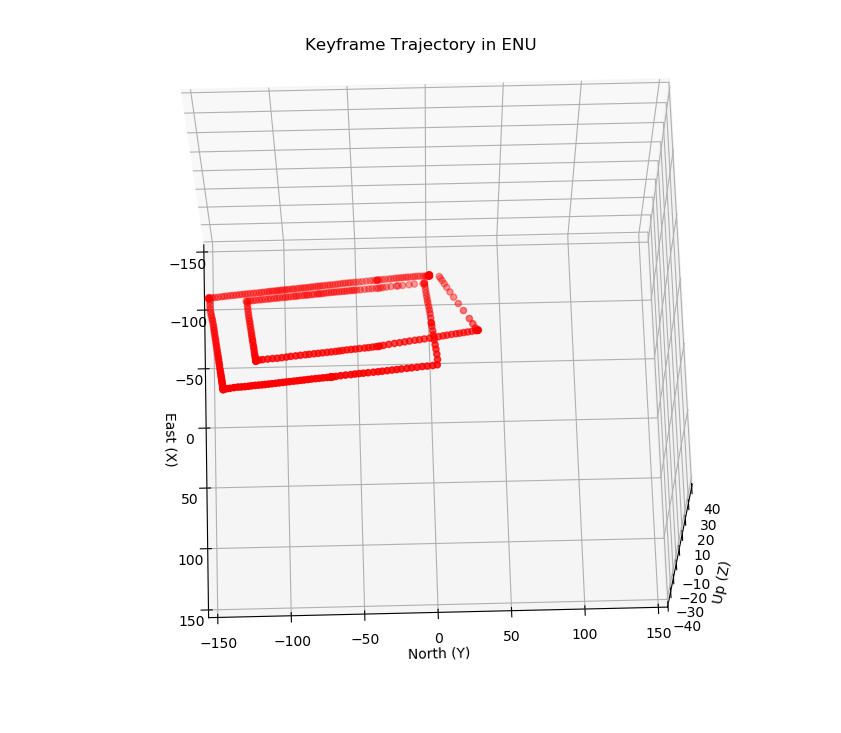
\includegraphics[height=12cm, width=15cm]{Images/KFTrajectoryENUwindowedTop.png}
    \caption{Point trajectory in ENU using window approach, Top view}
    \label{fig:kfgraphENUtop}
\end{figure}

Though initially, a disjoint set was selected from the list of elements by the window. This would omit 2 out of 3 elements from the selected scope and convert only the middle element. Later on, an overlapping window was used to select the window of elements resulting in full usage of all the points except couple of initial points which we were least interested in. The figures \ref{fig:kfgraphENUfront} and \ref{fig:kfgraphENUtop} are the results of an overlapping window approach and the scale is in meter (m).\\

Normal similarity transform method from colmap is enough to get a good transformation matrix estimation. But when we tested for multiple attempts, the estimation was not as expected. One of the cases where couple of points were estimated above the trajectory plane. For a real-time implementation like in our case, a more rigid estimation is required. Colmap also comes with a method that estimates transformation matrix using similarity transform with robust alignment.\\

Robust alignment uses RANSAC parameters to fit the closest and meaningful outcome for the transformation matrix. This helps in estimating the trajectory points more accurately and closer to actual point in real world scenario. The robust alignment addition was made in our static file data analysis and was tested on the same set of files for sanity. The similarity transform method in our gps\_process node was later on adapted to robust alignment.  

\section{Windowed approach for real-time processing}
\label{sec:windowapproachrealtime}
The real-time processing of the topics using the ros nodes vid\_orbslam3 and the gps\_process would yield the expected results and will prove the sanity of our approach discussed in the previous section. The overlapping windowed approach with robust alignment was added and adapted into our gps\_process node. For the real-time scenario, we do not have pre-defined points or keyframes in hand to slide over the whole set. The approach had to be modified to select the last N elements from the keyframe graph list and the ENU points list for the purpose of estimation of transformation matrix. N denotes the size of the window. The keyframes in the SLAM list were converted to ENU system and added onto a new list of keyframes. New keyframes to this list were added only when a new keyframe was available at the input /KeyframeGraphSLAM topic to avoid duplicate keyframes in the list. Further, the list of keyframes were published as a ros::PoseArray for further usage.\\

A static transform between ENU and ECEF (T\textsubscript{enu2ecef}) was also calculated using the initial ENU point after the lift off and was eventually published as a broadcast. This transform can be used by third-party tools and software to visualize the drone and camera poses on an earth-like environment by converting keyframe graph in ENU to earth scale.

\newpage

\section{Results}
\label{sec:results}
A simulation was executed using our nodes with recorded rosbag where the entire behaviour of the drone was captured. The following snapshots are the results of our implementation.

\begin{figure}[h]
    \centering
    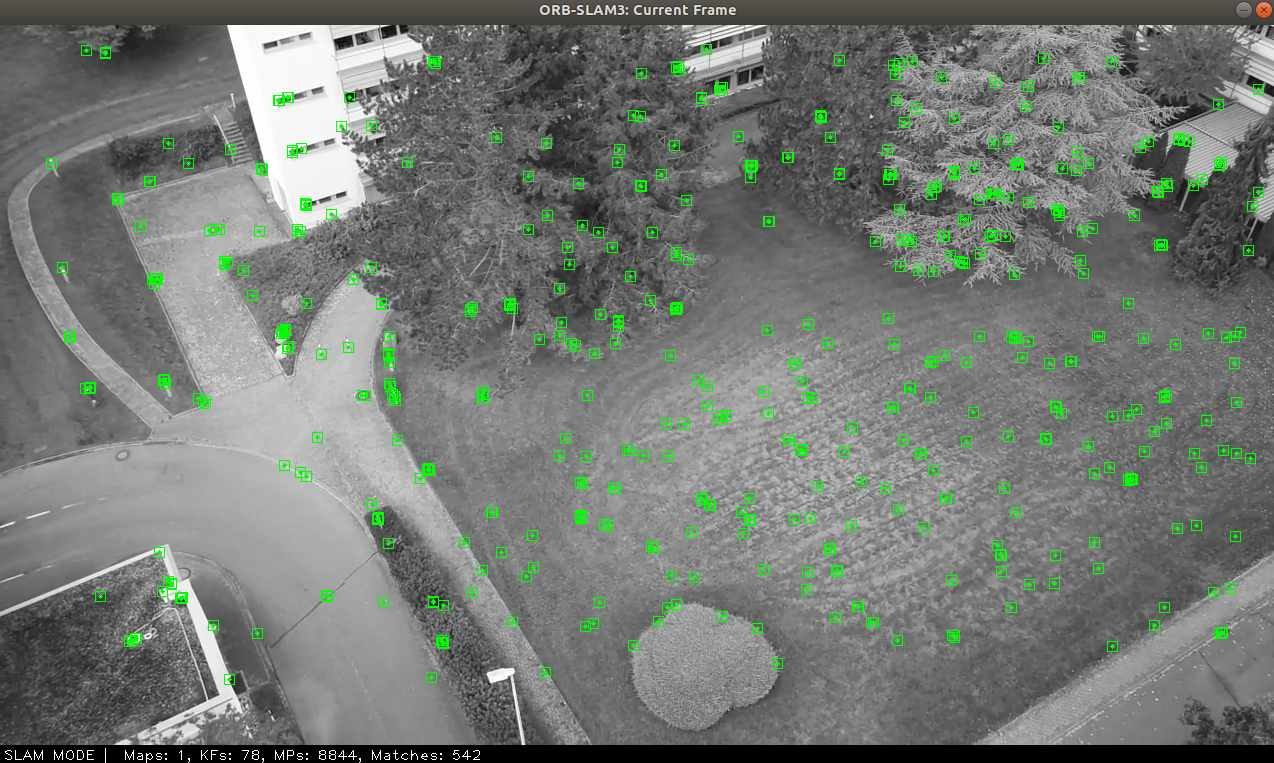
\includegraphics[height=6cm, width=12cm]{Images/camera_frame_orbslam3.png}
    \caption{Camera frame from orbslam3 visualization window.}
    \label{fig:cameraframe}
\end{figure}

\begin{figure}[h]
    \centering
    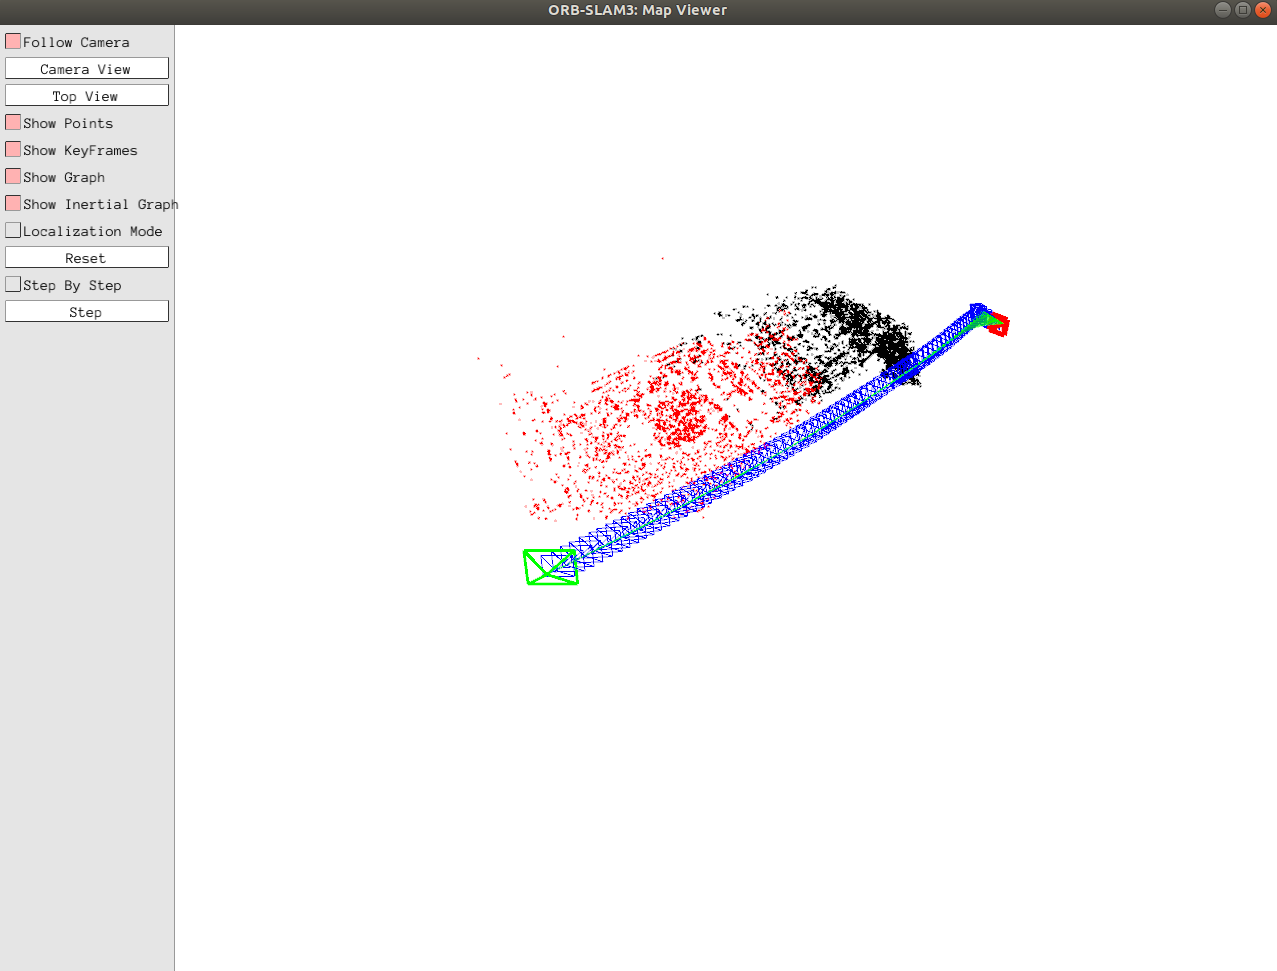
\includegraphics[height=6cm, width=12cm]{Images/trajectory_orbslam3.png}
    \caption{Keyframe trajectory atlas from orbslam3 visualization window.}
    \label{fig:kftrajatlas}
\end{figure}

The above figures \ref{fig:cameraframe} and \ref{fig:kftrajatlas} are the snapshots of the camera frame containing key points detected and the keyframe trajectory atlas depicting the current camera pose at a given instance of time. 

\begin{figure}[h]
    \centering
    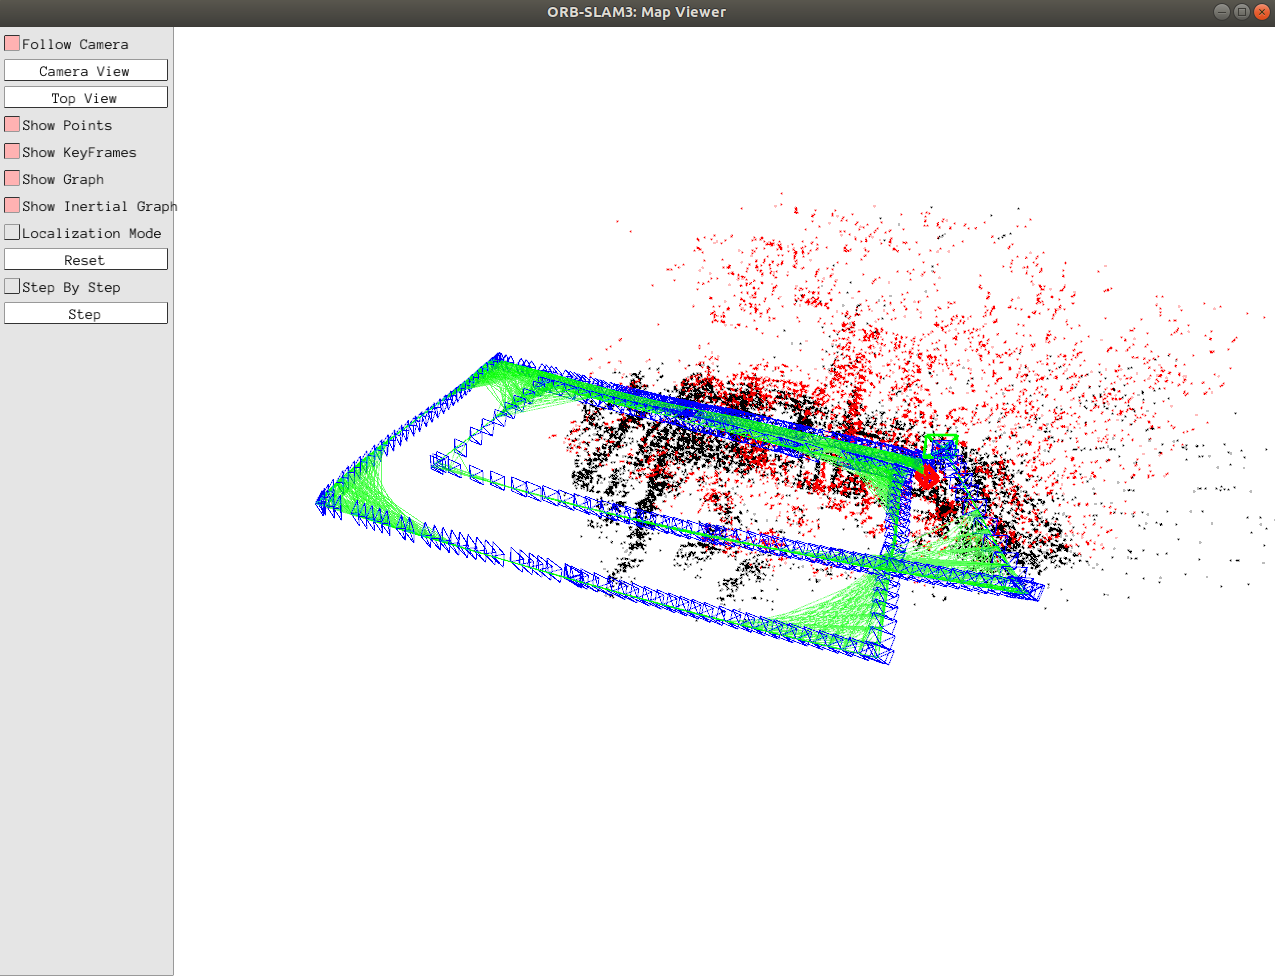
\includegraphics[height=6cm, width=12cm]{Images/trajectory_final_orbslam3.png}
    \caption{Complete Keyframe trajectory atlas from orbslam3 visualization window.}
    \label{fig:kftrajatlascomplete}
\end{figure}

The above figure \ref{fig:kftrajatlascomplete} shows the complete keyframe trajectory with the starting camera pose (red rectangle), detected key points, repeated key points and loop closure. The estimation of the above Visual SLAM depiction in ENU coordinate system resulting in a point trajectory is as shown in the following figures.

\begin{figure}[hbt!]
    \centering
    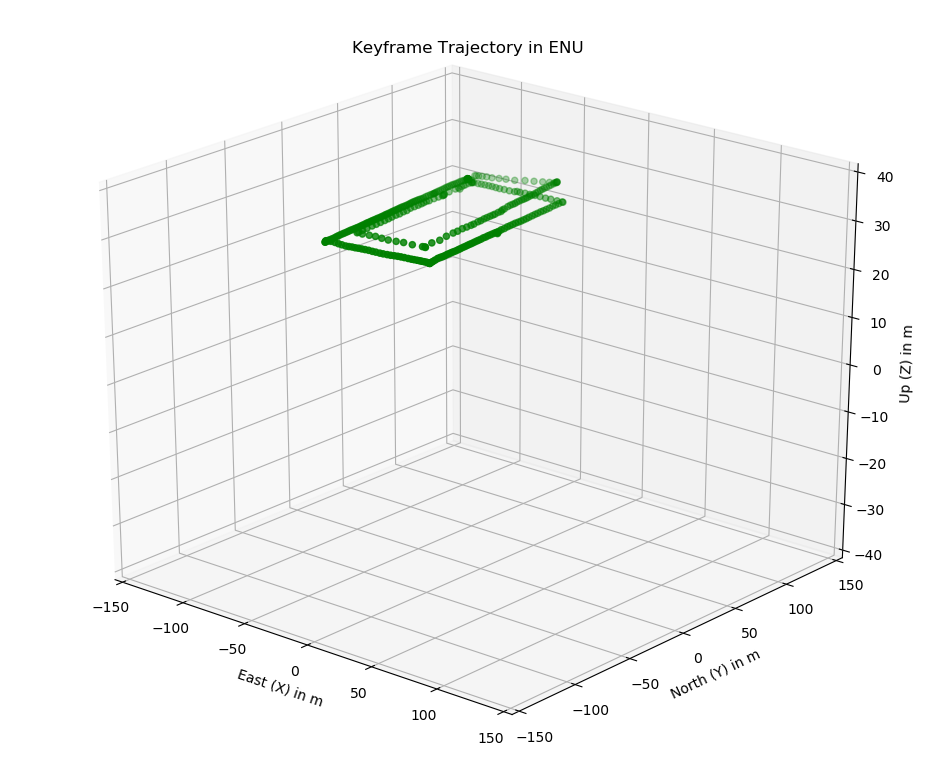
\includegraphics[height=9cm, width=13cm]{Images/kftrajectoryENUFinalIsometric.png}
    \caption{Point trajectory in ENU, Isometric view}
    \label{fig:kfgraphENUIsofinal}
\end{figure}

\begin{figure}[hbt!]
    \centering
    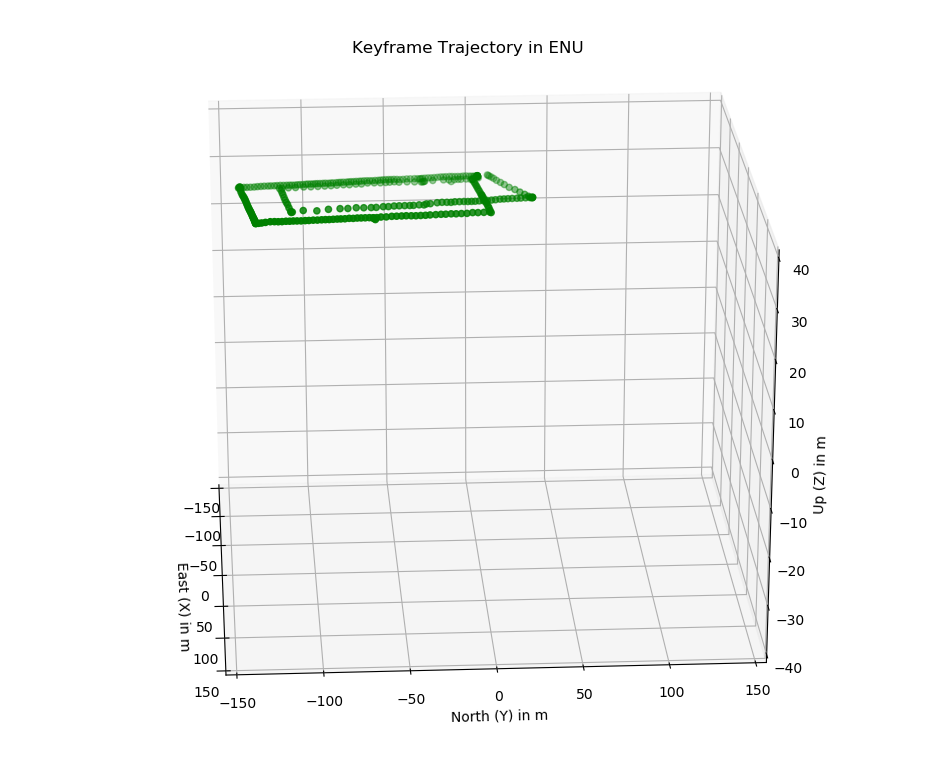
\includegraphics[height=9cm, width=13cm]{Images/kftrajectoryENUfinalFront.png}
    \caption{Point trajectory in ENU, Front view}
    \label{fig:kfgraphENUfrontfinal}
    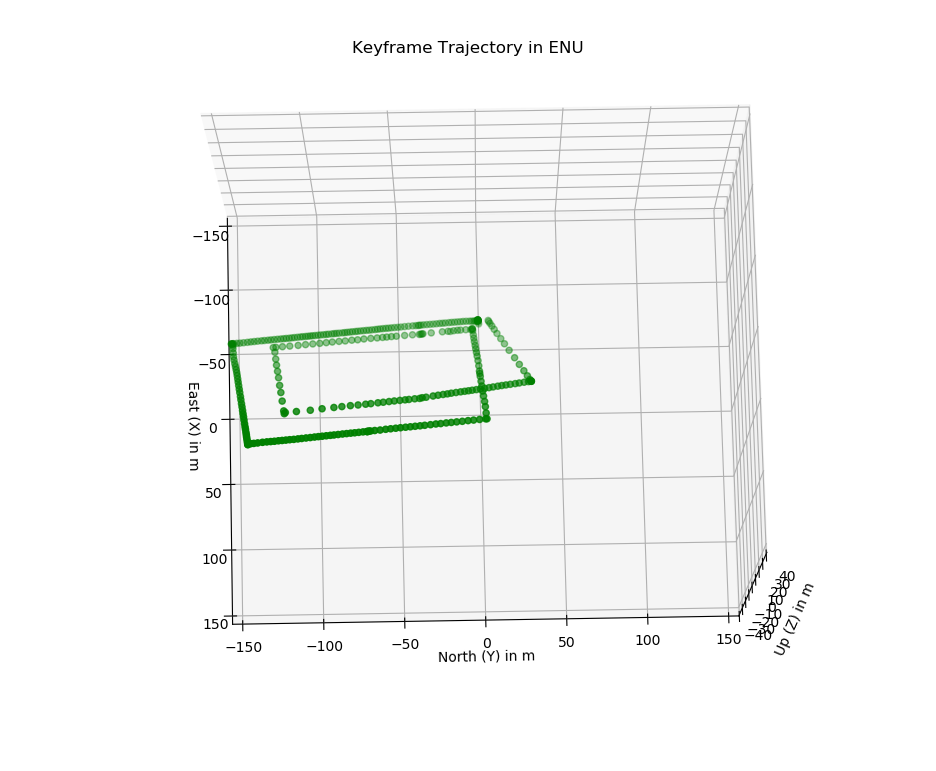
\includegraphics[height=9cm, width=13cm]{Images/kftrajectoryENUfinalTop.png}
    \caption{Point trajectory in ENU, Top view}
    \label{fig:kfgraphENUTopfinal}
\end{figure}

\newpage
We can clearly see the height of the flight at around 40 m above the grond in the Front view figure \ref{fig:kfgraphENUfrontfinal} which is the same height at which the drone flew. Even though the task is called as "Keyframe trajectory" estimation, the orientation visualization of the camera was not possible due to unknown issues with the format. An approach to correct this issue was planned but due to shortage of time duration in my internship the work was halted till this stage.

\section*{Additional task}
\section{Stereo rectification ROS node}
\label{sec:stereorectinode}
DJI Matrice 210 v2 RTK drone has stereo camera and provides many features in-built like disparity map, filtered disparity map and point cloud and also rectified image stream. Stereo rectification from the advanced sensing application of the drone requires CUDA support. Even though Manifold 2 supports CUDA, installing the DJI SDK and ROS SDK with CUDA dependency would drive the already hanging overhead to extreme level. \\

\begin{figure}[h]
    \centering
    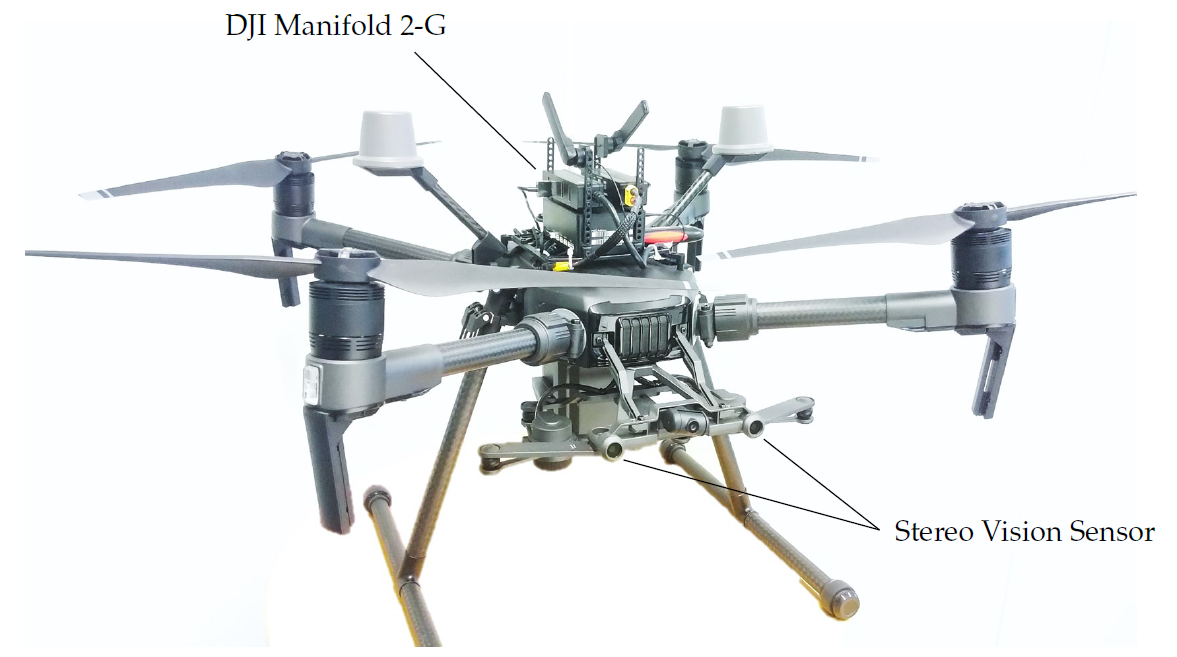
\includegraphics[width=11cm,height=7cm]{Images/djidronewithstereo.PNG}
    \caption{DJI Matrice 210 v2 RTK with integrated stereo vision sensor. Source: Mr Boitumelo Ruf}
    \label{fig:dronestereo}
\end{figure}

We wanted to develop a separate stand-alone node for the stereo image rectification. A ROS package named vid\_rectify \cite{vid_rectify} was developed to rectify the stereo images from the drone. The stereo cameras of the drone were calibrated and the stereo intrinsic parameter file was generated in OpenCV \cite{opencv_library} standard format. The node was tested and used in a project named "Real-time SGM Stereo Optimized for
Embedded ARM and CUDA Devices Mounted on Low-cost UAVs" authored by Mr Boitumelo Ruf and team. For an input rate of 20 fps, we obtained 20 fps output without any loss or frame drops in the process. The package is generic and compatible on any stereo setup. The documentation and the code base can be found in my github repository \cite{vid_rectify}.
 



\chapter{Conclusion}
\label{ch:conclusion}
Finally, at the end of this internship, I was able to develop a system of nodes which processes the real-time images and estimates camera poses and keyframe trajectory for a local ENU coordinate system and further can be extended to a global scale adapting it to ECEF coordinate system. For many reasons, my work may not be perfect but it has a lot of room for exploration and improvement. This report I would like to present gives an overall understanding on the tasks, challenges faced and development approaches that were carried out during the internship work. \\ 

This internship was an excellent and rewarding experience. During this course of work I have learnt the hard way by working on this platform. The internship gave me a great opportunity to explore new topics and skills and has made a identifiable growth in my scientific thinking and assertion skills. I believe my time spent in research and discovering new things was well worth it and contributed to the Fraunhofer Institute by finding acceptable solutions in a good way.
% ****************************************************************************************************
% Appendix
% ****************************************************************************************************
\appendix
\nocite{*} 
\bibliographystyle{plaindin}    
\bibliography{bibliography} 
\end{document}
